\documentclass[twoside,openright]{scrreprt}

\usepackage[msc]{tugrazthesis}
\usepackage{filecontents}  % for the integrated bibliography file (backwards compatibility)

\usepackage{algorithm}
\usepackage{algpseudocode}

\usepackage[american]{babel}
\usepackage[babel=true]{csquotes}
\usepackage[
    backend=biber,
    style=numeric,
]{biblatex}
\addbibresource{helper/references.bib}

\usepackage{tikz}
\usetikzlibrary{arrows.meta}
\usetikzlibrary{tikzmark,calc}
\usepackage{hyperref}
\usepackage{caption}
\usepackage[printonlyused]{acronym}
\usepackage{subcaption} % Add this in the preamble


\begin{document}
%My macros for making it easier to draw graphs 


% For 45° line -> center + 0.21
% For 22.5° line -> center.x + 0.27 , center.y + 0.11
% Cluster attacks -> cluster.y + 0.21 for top and - 0.21 for bottom
\newcommand{\DrawSelfAttackLeftTopCluster}[2]{% X, Y
\draw[-{To[length=4, width=5]}, line width=0.3mm] (#1, #2) 
.. controls (#1 -0.35, #2 + 0.34) and (#1 - 0.75, #2 - 0.12) .. 
(#1 - 0.13, #2 - 0.12);
}

\newcommand{\DrawAttackDiagonal}[5]{%Direction L.x L.y R.x R.y 
% Direction -> N = Negative slope LR = Left to Right
% Direction -> N = Negative slope RL = Right to Left
% Direction -> P = Positive slope LR = Left to Right
% Direction -> P = Positive slope RL = Right to Left
% Direction -> H = not 45° but Halfed=22.5°
\ifthenelse{\equal{#1}{NLR}}{
\draw[-{To[length=4, width=5]}, line width=0.3mm] (#2 + 0.21,#3 - 0.21) -- (#4 - 0.21 , #5 + 0.21);
}{
\ifthenelse{\equal{#1}{NRL}}{
\draw[-{To[length=4, width=5]}, line width=0.3mm] (#2 - 0.21,#3 + 0.21) -- (#4 + 0.21 , #5 - 0.21);
}{
\ifthenelse{\equal{#1}{PLR}}{
\draw[-{To[length=4, width=5]}, line width=0.3mm] (#2 + 0.21,#3 + 0.21) -- (#4 - 0.21 , #5 - 0.21);
}{
\ifthenelse{\equal{#1}{PRL}}{
\draw[-{To[length=4, width=5]}, line width=0.3mm]  (#2 - 0.21 , #3 - 0.21) -- (#4 + 0.21,#5 + 0.21);
}{}}}}}

\newcommand{\DrawAttackHorizontal}[5]{%Direction L.x L.y R.x R.y 
% R = Right to Left
% L = Left to Right
\ifthenelse{\equal{#1}{R}}{
\draw[-{To[length=4, width=5]}, line width=0.3mm] (#2 + 0.3,#3) -- (#4 - 0.3 , #5);
}{
\ifthenelse{\equal{#1}{L}}{
\draw[-{To[length=4, width=5]}, line width=0.3mm]  (#2 - 0.3,#3) -- (#4 + 0.3 , #5);
}{}}}


\newcommand{\DrawAttackVertical}[5]{%Direction L.x L.y R.x R.y 
% U = Down to Top
% D = Top to Down
% B = Double Attack
\ifthenelse{\equal{#1}{U}}{
\draw[-{To[length=4, width=5]}, line width=0.3mm] (#2,#3 + 0.3) -- (#4, #5 - 0.3);
}{
\ifthenelse{\equal{#1}{D}}{
\draw[-{To[length=4, width=5]}, line width=0.3mm] (#2,#3 - 0.3) -- (#4, #5 + 0.3);
}{
\ifthenelse{\equal{#1}{B}}{
\draw[-{To[length=4, width=5]}, line width=0.3mm] (#2 + 0.08, #3 - 0.3) -- (#4 + 0.08, #5 + 0.3);
\draw[{To[length=4, width=5]}-, line width=0.3mm] (#2 - 0.08, #3 - 0.3) -- (#4 - 0.08, #5 + 0.3);
}{}}}}

\definecolor{cBlue}{HTML}{004488}
\definecolor{cYellow}{HTML}{DDAA33}
\definecolor{cRed}{HTML}{BB5566}

%--- INFORMATION FOR TITLEPAGE -------------------------------------------------

% Your name including previous academic degrees (optional argument sets a different \author{}):
\thesisauthor[Firstname Lastname]{Christian Pasero, BSc}

% Title of your thesis (optional argument sets a different \title{}):
\thesistitle[Short Thesis Title]{Computation of Clustered\\Argumentation Frameworks via\\Boolean Satisfiability}

% Date of completion (optional argument sets a different \date{})
\thesisdate[ ]{\today}

% Supervisor headline (select male/female/plural version)
\supervisortitle{\germanenglish{Betreuer}{Supervisor}}

% Supervisor info
\supervisor{
Johannes P. Wallner, Ass.Prof. Dipl.-Ing. Dr.techn. BSc.\\
Institute of Software Technology
}


%\academicdegree{Diplom-Ingenieur/Diplom-Ingenieurin}
\academicdegree{Master of Science}

% Name of your degree programme according to your curriculum (only for msc/diplom
\curriculum{Computer Science}
%--- FRONT MATTER --------------------------------------------------------------

% Insert title page and affidavit

\printthesistitle

% 
\chapter*{Dev Notes}

\section{Concretizing less does not infer spuriousness}

\subsection{Concrete AF}

\begin{center}
	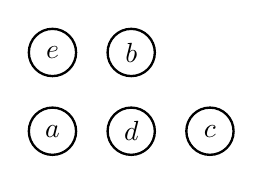
\begin{tikzpicture}
		\def \ax{0.0} \def \ay{-1.0}
		\def \bx{1.0} \def \by{0.0}
		\def \cx{2.0} \def \cy{-1.0}
		\def \dx{1.0} \def \dy{-1.0}
		\def \ex{0.0} \def \ey{0.0}
  
        % Singletons
        \draw[line width=0.3mm] (\ax,\ay)  circle (0.3) node[anchor=center]{$a$};
        \draw[line width=0.3mm] (\bx,\by)  circle (0.3) node[anchor=center]{$b$};
        \draw[line width=0.3mm] (\cx,\cy)  circle (0.3) node[anchor=center]{$c$};
        \draw[line width=0.3mm] (\dx,\dy)  circle (0.3) node[anchor=center]{$d$};
        \draw[line width=0.3mm] (\ex,\ey)  circle (0.3) node[anchor=center]{$e$};
		% Attacks
		\DrawAttackHorizontal{R}{\ex}{\ey}{\bx}{\by}
		\DrawAttackHorizontal{L}{\dx}{\dy}{\ax}{\ay}
		\DrawAttackHorizontal{R}{\dx}{\dy}{\cx}{\cy}

		\DrawAttackVertical{B}{\bx}{\by}{\dx}{\dy}
		\DrawSelfAttackRightSingleton{\bx}{\by}
		\DrawSelfAttackRightSingleton{\cx}{\cy}
        
	\end{tikzpicture}
\end{center}
\textbf{Stable Sets:} $\{ d, e\}$

\subsection{Abstract AF}
\begin{center}
	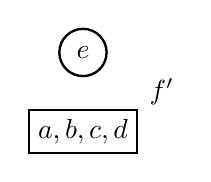
\begin{tikzpicture}
		\def \ex{0.0} \def \ey{ 0.0}
		\def \fx{0.0} \def \fy{-1.0}
        % Clusters
        \node[rectangle, draw, line width=0.3mm] at (\fx, \fy) {$a,b,c,d$};
		\node at (1, -0.5) {$f'$};
        % Singletons
        \draw[line width=0.3mm] (\ex,\ey)  circle (0.3) node[anchor=center]{$e$};
		% Attacks
		\DrawAttackVertical{U}{\fx}{\fy}{\ex}{\ey}
		\DrawSelfAttackLeftTopCluster{\fx-0.63}{\fy + 0.3}
	\end{tikzpicture}
\end{center}
\textbf{Stable Sets:} $\{ f', e\}$, $\{ e\}$

Abstract AF is \textbf{spurious} to concrete AF because set $\{ e\}$.



\subsection{Concretized AF (b,d) Grounded}
\begin{center}
	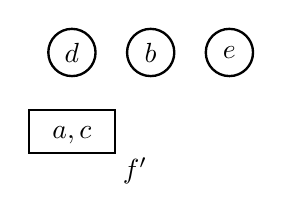
\begin{tikzpicture}
		\def \bx{1.0} \def \by{0.0}
		\def \dx{0.0} \def \dy{0.0}
		\def \ex{2.0} \def \ey{0}
		\def \fx{0.0} \def \fy{-1.0}
        % Clusters
        \node[rectangle, draw, line width=0.3mm] at (\fx, \fy) {$\phantom{d}a, c\phantom{d}$};
		\node at (0.8, -1.5) {$f'$};
        % Singletons
        \draw[line width=0.3mm] (\bx,\by)  circle (0.3) node[anchor=center]{$b$};
        \draw[line width=0.3mm] (\dx,\dy)  circle (0.3) node[anchor=center]{$d$};
        \draw[line width=0.3mm] (\ex,\ey)  circle (0.3) node[anchor=center]{$e$};
		% Attacks
		\DrawAttackHorizontal{B}{\bx}{\by}{\dx}{\dy}
		\DrawAttackHorizontal{R}{\bx}{\by}{\ex}{\ey}

		\DrawAttackVertical{D}{\dx}{\dy}{\fx}{\fy}

		\DrawSelfAttackRightSingleton{\bx}{\by}

		\DrawSelfAttackLeftTopCluster{\fx-0.45}{\fy + 0.3}
        
	\end{tikzpicture}
\end{center}
\textbf{Stable Sets:} $\{ d, e\}$, $\{ d, e, f'\}$

Concretized AF (b, d) is \textbf{spurious} to concrete AF because set $\{ d, e, f'\}$.


\subsection{Concretized AF (b)}
\begin{center}
	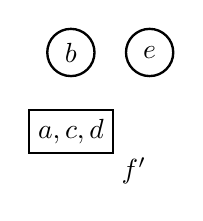
\begin{tikzpicture}
		\def \bx{0.0} \def \by{ 0.0}
		\def \ex{1.0} \def \ey{ 0.0}
		\def \fx{0.0} \def \fy{-1.0}
        % Clusters
        \node[rectangle, draw, line width=0.3mm] at (\fx, \fy) {$a,c,d$};
		\node at (0.8, -1.5) {$f'$};
        % Singletons
        \draw[line width=0.3mm] (\bx,\by)  circle (0.3) node[anchor=center]{$b$};
        \draw[line width=0.3mm] (\ex,\ey)  circle (0.3) node[anchor=center]{$e$};
		% Attacks
		\DrawAttackHorizontal{L}{\ex}{\ey}{\bx}{\by}
		\DrawAttackVertical{B}{\bx}{\by}{\fx}{\fy}

		\DrawSelfAttackRightSingleton{\bx}{\by}

		\DrawSelfAttackLeftTopCluster{\fx-0.45}{\fy + 0.3}
	\end{tikzpicture}
\end{center}
\textbf{Stable Sets:} $\{ f', e\}$

Concretized AF (e) is \textbf{faithful} to concrete AF.




% Other front matter you may want to include

\chapter*{Abstract}

English abstract of your thesis

\chapter*{Kurzfassung}

Deutsche Kurzfassung der Abschlussarbeit

% You will typically include *both a German and an English abstract*.
% The rest of the document will be either in German or in English.

\cleardoublepage

\chapter*{\germanenglish{Danksagung}{Acknowledgements}}

\germanenglish{Danke an alle, die beigetragen haben.}{Thanks to everyone who made this thesis possible}
% ...

\cleardoublepage

\tableofcontents

\listoffigures

\listoftables

%% HERE ACRONYMS
\chapter*{List of Acronyms and Symbols}


\newacro{AF} [AF] {Argumentation Framework}
\acrodefplural{AF}[AFs]{Argumentation Frameworks}

\newacro{AI} [AI] {Artificial Intelligence}
\newacro{ASP} [ASP] {Answer Set Programming}
\newacro{SAT-Solver} [SAT-Solver] {Boolean Satisfiability Solver}
\newacro{cf} [cf] {Conflict-Free}
\newacro{adm} [adm] {Admissible}
\newacro{stb} [stb] {Stable}
\newacro{BFS} [BFS] {Breadth First Search}
\newacro{DFS} [DFS] {Depth First Search}


\begin{acronym}[ICANN]
    \acro{AF} [AF] {Argumentation Framework}
    \acro{AI} [AI] {Artificial Intelligence}
    \acro{ASP} [ASP] {Answer Set Programming}
    \acro{cf} [cf] {Conflict-Free}
    \acro{adm} [adm] {Admissible}
    \acro{stb} [stb] {Stable}
    \acro{BFS} [BFS] {Breadth First Search}
    \acro{DFS} [DFS] {Depth First Search}
\end{acronym}



%--- MAIN CONTENT --------------------------------------------------------------

\chapter{Introduction}
% Argumentation in general and in research.
We all encounter arguments in our lives frequently. When talking to friends, listening to political discussions, or even making decisions in our head. These arguments can get heated and complex since humans have different beliefs and motivations. Finding a common ground or a ''correct`` conclusion is complicated and sometimes impossible. However, these imperfections are what make us humans. \ac{AI}, conversely, needs to act precisely and logically \cite{DBLP:journals/frai/DietzKM24}. To do so, the data needs to be stored and structured in a way, that AI can extract informations from it. This is part of knowledge representation and reasoning and that is why much research is being done in that field \cite{DBLP:journals/dagstuhl-manifestos/DelgrandeG0TW24, DBLP:journals/inffus/PopescuD23}.

% Abstraction of Argumentation -> promises and conclusions, attacks
Arguments can have many forms \cite{Toulmin_2003}. For instance, arguments can be seen as derivations of conclusions, based on assumptions or premises. Such premises can be facts or defeasible assumptions. Relations among arguments are key for driving (automated) argumentative reasoning. A prominent relation between arguments is that of an attack relation, or counter-argument relation. For instance, an argument might attack another. As an example, one argument might conclude that a square is red, while another is concluding that a square is blue. These two arguments are conflicting, and mutually attack each other. Another example would be that an argument is based on a witness statement, while a counter-argument to this one claims that the witness is not truthful, leading to a one-directional attack.



% Abstract Models of argumentation. Graphs.
If an argument $a$ is a counterargument of another argument $b$, we can say that $a$ attacks $b$. With this abstraction, we can abstract our model with directed graphs. The arguments are represented as nodes, and the attacks as directed edges \cite{DUNG1995321}. Now we can define argumentation frameworks (AFs) and use them to evaluate conclusions \cite{DBLP:conf/fapr/Geffner96}. In many cases, viewing arguments as abstract entities is sufficient to carry out argumentative reasoning. Such reasoning is defined via so-called argumentation semantics, which define criteria which (sets of) arguments are deemed jointly acceptable. One of the first pioneers in the topic of argumentation frameworks was Dung. He defined the structure and functionalities in 1995 \cite{Dung1995-DUNOTA-2}.

% Semantics with AFs
% Computation
Semantics define subsets of arguments that have a certain relation to each other. Dung defined different semantics \cite{Dung1995-DUNOTA-2} like conflict-free (cf), admissible (adm) and stable (stb). To be precise, conflict-free and admissible are semantical properties but we will treat them as semantics. According to Dung's definitions, a set \textit{S} is conflict-free if there are no attacks between the arguments in \textit{S}. The defintion of conflict-freeness is mainly a building block for the other semantics.
A stable extension, is a conflict-free set, if every argument, which is not in \textit{S}, has an attacker which is in \textit{S}.
Finally, an admissible set is a conflict-free set, where each argument in \textit{S} has a defender in \textit{S}. A defender is this context means an argument which attacks an attacker of an argument in \textit{S}.


% Clustering of AFs
Since AFs can get very big and complicated, another layer of abstraction can be added. This abstraction layer is called \emph{clustering} and generalizes multiple arguments into one bundled cluster \cite{DBLP:conf/kr/SaribaturW21}. In this thesis we refer to the clustered AF as \emph{abstract AF} and the original AF, where no clustering occurs is called \emph{concrete AF}.
Clustering of arguments is a technique to reduce the number of arguments and to provide a high-level view of a given AF. Here, clustering means that arguments can be clustered together in clusters (or clustered arguments). In general, as is the case with many abstraction techniques, clustering can change conclusions that can be drawn from an abstracted formalism. A clustering is said to be \emph{faithful} if no erroneous conclusions can be drawn that is not part of the original, non-abstracted, structure. Otherwise, if conclusions can be drawn that are not there on the original structure, we say that these are \emph{spurious} conclusions.

In our case, the semantics of conflict-free, admissibility, and stable semantics were "lifted`` to the case with clustered arguments. That is, a clustered (abstracted) version of conflict-free sets, admissible sets, and stable extensions was defined on clustered AFs. These semantics respect the clustering of arguments. Then, e.g., an abstract admissible set is spurious if there is no (concrete, non-abstract) admissible set matching this one in the concrete AF. If no such spurious sets exist, then the clustered AF is said to be faithful, w.r.t.\ the concrete AF.






% Example
For instance, let us consider a real-world example like the weather. We can define arguments.

\begin{itemize}
    \item $a$: The sky is blue.
    \item $b$: The atmosphere scatters the sunlights and makes the sky appear blue.
    \item $c$: There exist photographs of a blue sky.
    \item $d$: Photographs can be fake.
    \item $e$: At sunrise the sky appears to be orange.
    \item $f$: Observations can alter, depending on the time.
\end{itemize}

With this knowledge basis, we can create a concrete AF $G=(A, R)$. Where we abstract the arguments into nodes and transform the opposing statement into attacks as shown in \cref{af:introExample1}. An opposing statement in this context would be for instance the argument $a$ (i.e.\ \emph{The sky is blue}) and $e$ (i.e.\ \emph{At sunrise the sky appears to be orange}). Since both statements can not be true at the same time, they are contradicting, or in other words, attacking each other. If we apply another layer of abstraction, we obtain, e.g.\ the abstract AF $\hat{G}=(\hat{A}, \hat{R})$ defined in \cref{af:introExample2}. We call arguments which are clustered, \emph{clustered arguments} and arguments which are not in clusters \emph{singletons}. Here, we created a single cluster consisting of the arguments $\{a, b, c, e, f\}$.



\vspace{0.3cm}
\begin{figure}[h]
    \centering
    \begin{minipage}{.5\textwidth}
        \centering
        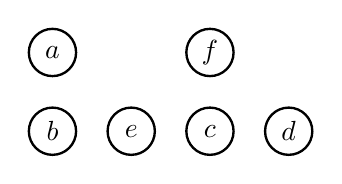
\begin{tikzpicture}
            % Singletons
            \def \ax{0}     \def \ay{0}
            \def \bx{0}     \def \by{-1}
            \def \cx{2}     \def \cy{-1}
            \def \dx{3}     \def \dy{-1}
            \def \ex{1}     \def \ey{-1}
            \def \fx{2}     \def \fy{0}

            \draw[line width=0.3mm] (\ax, \ay) circle (0.3) node[anchor=center]{$a$};
            \draw[line width=0.3mm] (\bx, \by) circle (0.3) node[anchor=center]{$b$};
            \draw[line width=0.3mm] (\cx, \cy) circle (0.3) node[anchor=center]{$c$};
            \draw[line width=0.3mm] (\dx, \dy) circle (0.3) node[anchor=center]{$d$};
            \draw[line width=0.3mm] (\ex, \ey) circle (0.3) node[anchor=center]{$e$};
            \draw[line width=0.3mm] (\fx, \fy) circle (0.3) node[anchor=center]{$f$};

            % Attacks
            \DrawAttackHorizontal{L}{\fx}{\fy}{\ax}{\ay}
            \DrawAttackHorizontal{B}{\ex}{\ey}{\bx}{\by}
            \DrawAttackHorizontal{B}{\cx}{\cy}{\ex}{\ey}
            \DrawAttackHorizontal{L}{\dx}{\dy}{\cx}{\cy}
            \DrawAttackVertical{D}{\fx}{\fy}{\cx}{\cy}
            \DrawAttackDiagonal{PB}{\fx}{\fy}{\ex}{\ey}
            \DrawAttackDiagonal{NB}{\ax}{\ay}{\ex}{\ey}
        \end{tikzpicture}
        \subcaption{Concrete AF $G$}
        \label{af:introExample1}
    \end{minipage}%
    \begin{minipage}{.5\textwidth}
        \centering
        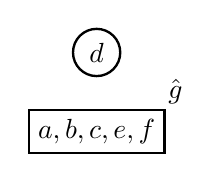
\begin{tikzpicture}
            % Singletons
            \def \gx{0}     \def \gy{-1}
            \def \dx{0}     \def \dy{0}

            \node[rectangle, draw, line width=0.3mm] at (\gx, \gy) {$a,b,c,e,f$};
            \node at (1, -0.5) {$\hat{g}$};
            \draw[line width=0.3mm] (\dx, \dy) circle (0.3) node[anchor=center]{$d$};

            % Attacks
            \DrawSelfAttackLeftTopCluster{\gx-0.8}{\gy + 0.3}
            \DrawAttackVertical{D}{\dx}{\dy}{\gx}{\gy}
        \end{tikzpicture}
        \subcaption{Abstract AF $\hat{G}$}
        \label{af:introExample2}
    \end{minipage}
    \caption{Concrete and abstract AF}
    \label{fig:comparison}
\end{figure}





Now we can compute the sets of the according semantics (cf, adm, stb). The definitions of the semantics are defined in the \cref{ch:Background}. To reduce cluttering, we keep this example to the stable semantics. The stable extensions of the AF $G$ are $\mathtt{stb=}\bigl\{\{d, e\}, \{b, d, f\}\bigl\}$.

By computing the stable extensions of the abstract AF $\hat{G}$ $\mathtt{stb=}\bigl\{\{d\}, \{d, \hat{g}\}\bigl\}$, we can observe that the AF is spurious due to the extension $\{d\}$, since the abstract stable extension cannot be mapped to one of the concrete stable extensions.

When concretizing (i.e. removing an argument from the cluster) the argument $c$, we create a new AF $\hat{G}' = (\hat{A}', \hat{R}')$ depicted in \cref{af:introExample3}, which has the following stable extensions $\mathtt{stb=}\{\hat{g}, d\}$. This extension can be mapped to both stable extensions of the concrete AF $G$, by mutating the cluster $\hat{g}$ with $\{e\}$ or $\{b, f\}$. Thus, we created a faithful abstract AF.

\begin{figure}[h]
    \centering
    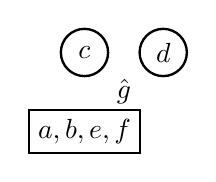
\begin{tikzpicture}
        % Singletons
        \def \gx{0}     \def \gy{-1}
        \def \dx{1}     \def \dy{0}
        \def \cx{0}     \def \cy{0}

        \node[rectangle, draw, line width=0.3mm] at (\gx, \gy) {$a,b,e,f$};
        \node at (0.5, -0.5) {$\hat{g}$};
        \draw[line width=0.3mm] (\dx, \dy) circle (0.3) node[anchor=center]{$d$};
        \draw[line width=0.3mm] (\cx, \cy) circle (0.3) node[anchor=center]{$c$};

        % Attacks
        \DrawSelfAttackLeftTopCluster{\gx-0.65}{\gy + 0.3}
        \DrawAttackHorizontal{L}{\dx}{\dy}{\cx}{\cy}
        \DrawAttackVertical{B}{\cx}{\cy}{\gx}{\gy}
    \end{tikzpicture}
    \caption{Concretized AF $\hat{G}'$}
    \label{af:introExample3}
\end{figure}


% Importance of concretizing single arguments
When producing an AF with multiple layer of abstractions, we obtain a high-level view of the concrete AF. This simplification has the drawback to lose some details. To still have a deep understanding of the structure to some extend, extracting single arguments of the cluster by concretizing them can be helpful. This also allows the user to have a direct impact to the outcome and produce customized faithful AFs.


% What we want to show in this paper
% Main contributions in this paper
%Complexity
Creating abstract, faithful AFs can be challenging and is the main focus of this thesis. Unfortunately, drawing a conclusion from an AF can be challenging, e.g., it can be NP-complete and sometimes even be beyond NP to decide whether an argument is acceptable under a specific argumentation semantics \cite{DBLP:journals/ai/DvorakGRW23}. In fact, the complexity of proving faithfulness or spuriousness of an AF is $\prod_2^P$ hard \cite{DBLP:conf/kr/SaribaturW21}. In practice, this means, that to obtain a result, multiple instances or calls of a SAT-Solver need to be invoked.

We created one of the first tools to produce an abstract AFs based on a concrete AFs. We cover different setups and usages, including different semantics and base functionalities. The main contributions of this thesis are as follows.

\begin{itemize}
    \item We provide algorithms for computing abstract semantics of a given clustered AF. That is, our algorithms are capable of computing or enumerating all extensions under abstract conflict-free, admissible, and stable semantics.

    \item Based on our algorithms for computing abstract semantics, we provide algorithmic solutions for checking faithfulness of a given clustered AF. We develop two approaches in this regard: (i) one of based on breadth-first-search (BFS) and (ii) one based on depth-first search (DFS). While the algorithm based on BFS first calculates all original extensions and abstract extensions of a given AF and clustered AF, respectively, the DFS variant iteratively computes abstract extensions of the clustered AF and verifies (non-)spuriousness of this extension.

    \item Towards user-interaction, for a given AF and clustered AF, we provide an algorithm for concretization, by which we mean that a user can select arguments inside clusters to be made concrete (singletons). We then refine the clustered AF until faithfulness is reached, since the extraction of the user-defined arguments may result in spurious reasoning.
    
    \item We implemented our algorithms in TODO how? and provide the implementations in open-source.
    \item In an experimental evaluation, $\cdots$ TODO results.
    \item $\cdots$
\end{itemize}

We provide an open source implementation of the previously listed tools \cite{Pasero2024-AFClustering-Repo}.

\begin{center}
    \url{https://github.com/p4s3r0/argumentation-framework-clustering}
\end{center}

\noindent

\textit{TODO: Further contributions}

\textit{TODO: Choice of methods to obtain results}

\textit{TODO: How big AFs are still feasible to solve}


\chapter{Background}

\section{Argumentation Frameworks}


Argumentation frameworks were first formally described by Dung in 1995 \cite{DUNG1995321}. They represent an information state, where various conclusions can be drawen from. An AF $G = (A, R)$ consists of two parameters: a set of arguments $A$, and a collection of relations $R$, called attacks which describe the conflicts between the arguments.

They are mostly used in the fields of \ac{AI}, f.e. in automated reasoning and logic programming \cite{AFINAIARLP, AFINAIARLPexample}. But do also find their applications in other fields like Natural Language Processing \cite{AFINNLP}, Trust and Reputation Systems \cite{AFINTaRS}, and even in Game Theory and Strategic Reasoning \cite{AFinGames}.

AFs are represented by directed graph, where the nodes are an abstraction of the arguments $A$, and the arrows represent the attacks $R$. Let us define an AF $G = (A, R)$ with the arguments
$\mathtt{A=\{a, b, c, d, e\}}$ and the attacks
$\mathtt{R=[(a,b),}$
$\mathtt{(b,b),}$
$\mathtt{(a,c),}$
$\mathtt{(c,a),}$
$\mathtt{(c,d),}$
$\mathtt{(d,e),}$
$\mathtt{(e,d)]}.$

With the arguments and attacks, we can create a directed graph \ref{af:backgroundAFexample1}.
\begin{figure}[h]
    \centering
    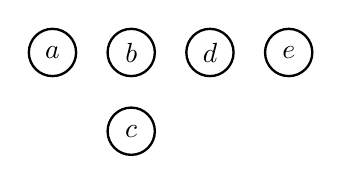
\begin{tikzpicture}
        % Singletons
        \def \ax{0}     \def \ay{0}
        \def \bx{1}     \def \by{0}
        \def \cx{1}     \def \cy{-1}
        \def \dx{2}     \def \dy{0}
        \def \ex{3}     \def \ey{0}

        \draw[line width=0.3mm] (\ax, \ay) circle (0.3) node[anchor=center]{$a$};
        \draw[line width=0.3mm] (\bx, \by) circle (0.3) node[anchor=center]{$b$};
        \draw[line width=0.3mm] (\cx, \cy) circle (0.3) node[anchor=center]{$c$};
        \draw[line width=0.3mm] (\dx, \dy) circle (0.3) node[anchor=center]{$d$};
        \draw[line width=0.3mm] (\ex, \ey) circle (0.3) node[anchor=center]{$e$};

        % Attacks
        \DrawAttackHorizontal{R}{\ax}{\ay}{\bx}{\by}
        \DrawSelfAttackRightSingleton{\bx}{\by}
        \DrawAttackDiagonal{NB}{\ax}{\ay}{\cx}{\cy}
        \DrawAttackDiagonal{PLR}{\cx}{\cy}{\dx}{\dy}
        \DrawAttackHorizontal{B}{\ex}{\ey}{\dx}{\dy}
    \end{tikzpicture}
    \caption{\ac{AF} G}
    \label{af:backgroundAFexample1}
\end{figure}

To be able to conclude something, out of an abstract AF, we need to define semantics. A semantic defines a subset of argument sets that satisfy the semantic-specific rules. Dung already defined different semantics \cite{Dung1995-DUNOTA-2} like conflict-free, admissible and stable.

\paragraph{conflict-free:} According to Dungs definitions, a set \textit{S} is conflict-free if there are no attacks between the arguments in \textit{S}. Or, formally:

\begin{center}
    \begin{tabular}{c}
        $S \in cf(G)$ \textit{iff for each} $a, b \in S$ \textit{we have} $(a, b) \not\in R$
    \end{tabular}
\end{center}

The conflict-free set is mainly a building block for the other semantics, which means that the conflict-free set is always a superset of admissible and stable.

In the example \ref{af:backgroundAFexample1} the conflict-free sets are:
$\mathtt{\{a\}},$
$\mathtt{\{c\}},$
$\mathtt{\{d\}},$
$\mathtt{\{e\}},$
$\mathtt{\{a, d\}},$
$\mathtt{\{a, e\}},$
$\mathtt{\{c, e\}},$

\paragraph{admissible:} An admissible set is a conflict-free set, where each argument in \textit{S} has a defender in \textit{S}. Or, formally:

\begin{center}
    \begin{tabular}{c}
        $S \in adm(G)$ \textit{iff} $S \in cf(G)$\\

        \textit{and if} $a \in S$ \textit{with} $(b, a) \in R$,\\

        \textit{then there is a} $c \in G$ \textit{with} $(c, b) \in R$
    \end{tabular}
\end{center}

In the example \ref{af:backgroundAFexample1} the $admissible$ sets are:
$\mathtt{\{a\}},$
$\mathtt{\{c\}},$
$\mathtt{\{e\}},$
$\mathtt{\{a, d\}},$
$\mathtt{\{a, e\}},$
$\mathtt{\{c, e\}}$


\paragraph{stable:} A stable set is a conflict-free set, if for every argument, which is not in \textit{S}, there exists an attacker in \textit{S}. Or, formally:

\begin{center}
    \begin{tabular}{c}
        $S \in stb(G)$ \textit{iff} $S \in cf(G),  b \not\in S$ \textit{implies}\\

        \textit{that there is an} $a \in S$ \textit{with} $(a, b) \in R$,\\

        \textit{and if} $S$ \textit{does not attack an} $a \in S$ \textit{then} $b \not\in S$\\

        \textit{whenever} $(a, b) \in R$ \textit{and singleton}$(b)$
    \end{tabular}
\end{center}


 In the example \ref{af:backgroundAFexample1} the $stable$ sets are:
$\mathtt{\{a, d\}},$
$\mathtt{\{a, e\}}$

\vspace{0.5cm}
\noindent
The specific semantic rules can also be defined via a boolean formula. Which then can be used to encode the AFs to be solvable with different boolean solvers like \ac{ASP} \cite{DBLP:journals/corr/abs-1301-1388} or, as in our case, with a \ac{SAT-Solver} \cite{DBLP:journals/amai/AmgoudD13}. Unfortunately, drawing a conclusion from an AF can be challenging, e.g., it can be NP-complete and sometimes even be beyond NP to decide whether an argument is acceptable under a specific argumentation semantics \cite{DBLP:journals/ai/DvorakGRW23}.



\section{Clustering of Argumentation Frameworks}

When talking about AFs in general, we already have an abstraction layer due to the arguments abstraction. By clustering, we add another layer of abstraction where we combine different arguments into one or multiple so called \textit{clusters}. The arguments which are not clustered are called \textit{singletons}.
By definition, a cluster is a single entity (composed of multiple arguments) which can be integrated in an AF to reduce the complexity. While reducing the overall complexity of the AF with clusters, we add a new computation layer: Computing \textit{faithful} clustered AFs. The term \textit{faithful} describes the property of a clustered AF, that every abstract semantic extension can be mapped to a concrete semantic extension. If the clustered AF creates a semantic set which cannot be mapped to a concrete set, we call it \textit{spurious}.

Clustered abstract AFs can also be model with graphs. Where each argument is a node, every attack an arrow and each cluster is represented with a rectangle with every clustered argument inside of it. Let us have a look at an example and define AF $\mathtt{\hat{G}=(\hat{A}, \hat{R})}$ with the arguments $\mathtt{\hat{A}=\{d, e, \hat{h}\}}$ and the attacks $\mathtt{[(\hat{h}, d), (d, e), (e, d), (\hat{h}, \hat{h})]}$. With this definition we can create the directed graph \ref{af:backgroundExampleClusterSpurious}.


\begin{figure}[h]
    \centering
    
\begin{tikzpicture}
        % Singletons
        \def \ex{3}     \def \ey{0}
        \def \dx{2}     \def \dy{0}
        \def \hx{0}     \def \hy{0}

        \node[rectangle, draw, line width=0.3mm] at (\hx, \hy) {$a,b,c,d$};
        \node at (0, 0.55) {$\hat{h}$};
        \draw[line width=0.3mm] (\ex, \ey) circle (0.3) node[anchor=center]{$e$};
        \draw[line width=0.3mm] (\dx, \dy) circle (0.3) node[anchor=center]{$d$};

        % Attacks
        \DrawSelfAttackLeftTopCluster{\hx-0.65}{\hy + 0.3}
        \DrawAttackHorizontal{R}{\hx+0.5}{\hy}{\dx}{\dy}
        \DrawAttackHorizontal{B}{\ex}{\ey}{\dx}{\dy}
    \end{tikzpicture}
    \caption{\ac{AF} $\hat{G}$ clustered}
    \label{af:backgroundExampleClusterSpurious}
\end{figure}


%\textit{TODO: Definition of Semantics}
Since clusters can not be treated the exact same way as an argument, we need to refine the semantic definitions. Let us consider a clustered AF $\mathtt{\hat{G}=\{\hat{A}, \hat{R}\}}$ and redefine the following semantics:
\paragraph{conflict-free:} A set of arguments is conflict-free, if there is no attack between the singletons of the set. Or, formally, as specified in \cite{DBLP:conf/kr/SaribaturW21}:

\begin{center}
    \begin{tabular}{c}
        $\hat{S} \in \hat{cf}(\hat{G})$ \textit{iff for each} $\hat{a}, \hat{b} \in$ \textit{singleton}($\hat{S}$) \textit{we have} $(\hat{a}, \hat{b}) \not\in \hat{R}$.
    \end{tabular}
\end{center}

In the example \ref{af:backgroundExampleClusterSpurious} the conflict-free sets are:
$\mathtt{\{d}\}$,
$\mathtt{\{e}\}$,
$\mathtt{\{\hat{h}}\}$,
$\mathtt{\{e, \hat{h}}\}$,
$\mathtt{\{d, \hat{h}}\}$



\paragraph{admissible:} A set of arguments is admissible, if it is conflict-free and if every singleton which is being attacked, has a defender. Or, formally, as specified in \cite{DBLP:conf/kr/SaribaturW21}:

\begin{center}
    \begin{tabular}{c}
        $\hat{S} \in \hat{adm}(\hat{G})$ \textit{iff} $\hat{S} \in \hat{cf}(\hat{G})$\\

        \textit{and if} $\hat{a} \in \hat{S}$ \textit{with} $(\hat{b}, \hat{a}) \in \hat{R}$ \textit{with singleton}($\hat{a}$),\\

        \textit{then there is a} $\hat{c} \in \hat{G}$ \textit{with} $(\hat{c}, \hat{b}) \in \hat{R}$
    \end{tabular}
\end{center}

In the example \ref{af:backgroundExampleClusterSpurious} the admissible sets are:
$\mathtt{\{e}\}$,
$\mathtt{\{\hat{h}}\}$,
$\mathtt{\{e, \hat{h}}\}$,
$\mathtt{\{d, \hat{h}}\}$



\paragraph{stable:} A set of arguments is stable, if it is conflict-free and if an argument is not in the stable set, it implies that an argument in the stable set is attacking it. Furthermore if the stable set is not attacking an argument, then every singleton attacking the argument is not in the stable set. Or, formally, as specified in \cite{DBLP:conf/kr/SaribaturW21}:
\begin{center}
    \begin{tabular}{c}
        $\hat{S} \in \hat{stb}(\hat{G})$ \textit{iff} $\hat{S} \in \hat{cf}(\hat{G}),  \hat{b} \not\in \hat{S}$ \textit{implies}\\

        \textit{that there is an} $\hat{a} \in \hat{S}$ \textit{with} $(\hat{a}, \hat{b}) \in \hat{R}$,\\

        \textit{and if} $\hat{S}$ \textit{does not attack an} $\hat{a} \in \hat{S}$ \textit{then} $\hat{b} \not\in \hat{S}$\\

        \textit{whenever} $(\hat{a}, \hat{b}) \in \hat{R}$ \textit{and singleton}$(\hat{b})$
    \end{tabular}
\end{center}

In the example \ref{af:backgroundExampleClusterSpurious} the admissible sets are:
$\mathtt{\{e, \hat{h}}\}$,
$\mathtt{\{d, \hat{h}}\}$

\vspace{0.5cm}
\noindent
Let us have a look at a concrete example to explain faithfulness. The concrete AF $G = (A, R)$ has the following arguments $\mathtt{A=\{a, b, c, d, e\}}$ with these attacks:
$\mathtt{R=[(a,b),}$
$\mathtt{(b,b),}$
$\mathtt{(a,c),}$
$\mathtt{(c,a),}$
$\mathtt{(c,d),}$
$\mathtt{(d,e),}$
$\mathtt{(e,d)]}$.

With this definition we can define the graph \textit{G} in \ref{af:backgroundClusterExample1}.

Now we can group the arguments $\mathtt{\{a, b, c, d\}}$ together into one single cluster $\mathtt{\hat{h}}$. The arguments for the abstract AF $\mathtt{\hat{H} = (\hat{B}, \hat{S})}$ would then be $\mathtt{\hat{B}=\{e, \hat{h}\}}$ with the according attacks:
$\mathtt{\hat{S}=[(\hat{h}, e), (e, \hat{h}), (\hat{h}, \hat{h})]}$

With this defintion we can build the abstract clustered graph $\mathtt{\hat{H}}$ in \ref{af:backgroundClusterExample2}


\vspace{0.3cm}
\begin{figure}[h]
\begin{minipage}{.5\textwidth}
    \centering
    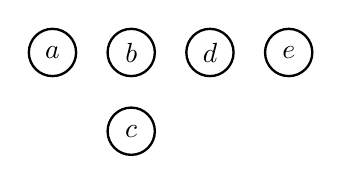
\begin{tikzpicture}
        % Singletons
        \def \ax{0}     \def \ay{0}
        \def \bx{1}     \def \by{0}
        \def \cx{1}     \def \cy{-1}
        \def \dx{2}     \def \dy{0}
        \def \ex{3}     \def \ey{0}

        \draw[line width=0.3mm] (\ax, \ay) circle (0.3) node[anchor=center]{$a$};
        \draw[line width=0.3mm] (\bx, \by) circle (0.3) node[anchor=center]{$b$};
        \draw[line width=0.3mm] (\cx, \cy) circle (0.3) node[anchor=center]{$c$};
        \draw[line width=0.3mm] (\dx, \dy) circle (0.3) node[anchor=center]{$d$};
        \draw[line width=0.3mm] (\ex, \ey) circle (0.3) node[anchor=center]{$e$};

        % Attacks
        \DrawAttackHorizontal{R}{\ax}{\ay}{\bx}{\by}
        \DrawSelfAttackRightSingleton{\bx}{\by}
        \DrawAttackDiagonal{NB}{\ax}{\ay}{\cx}{\cy}
        \DrawAttackDiagonal{PLR}{\cx}{\cy}{\dx}{\dy}
        \DrawAttackHorizontal{B}{\ex}{\ey}{\dx}{\dy}
    \end{tikzpicture}
    \caption{\ac{AF} G}
    \label{af:backgroundClusterExample1}
\end{minipage}%
\begin{minipage}{.5\textwidth}
    \centering
    
\begin{tikzpicture}
        % Singletons
        \def \ex{2}     \def \ey{0}
        \def \hx{0}     \def \hy{0}

        \node[rectangle, draw, line width=0.3mm] at (\hx, \hy) {$a,b,c,d$};
        \node at (0, 0.55) {$\hat{h}$};
        \draw[line width=0.3mm] (\ex, \ey) circle (0.3) node[anchor=center]{$e$};

        % Attacks
        \DrawSelfAttackLeftTopCluster{\hx-0.65}{\hy + 0.3}
        \DrawAttackHorizontal{B}{\ex}{\ey}{\hx+0.5}{\hy}
    \end{tikzpicture}
    \caption{\ac{AF} $\hat{H}$ clustered}
    \label{af:backgroundClusterExample2}
\end{minipage}
\end{figure}

If we compare the stable sets of the concrete AF $G$ (e.g. $\mathtt{stb=[\{a, e\}, \{a, d\}]}$) with the stable sets of the abstract clustered AF $\hat{H}$ (e.g. $\mathtt{\hat{stb}=[\{\hat{h}\}, \{e\}, \{e, \hat{h}\}]}$), we see that it is spurious due to the stable set $\mathtt{\{e\}}$ which cannot be mapped to one of the concrete stable sets. To create a faithful clustered AF, we need to concretize one or more arguments of the cluster. By concretizing the argument $\mathtt{\{d\}}$, we obtain a new AF $\hat{I}=(\hat{B}, \hat{T})$ with the arguments $\mathtt{\hat{B}=\{d, e, \hat{h}\}}$ and the attacks $\mathtt{\hat{T}=[(d, \hat{h}),}$
$\mathtt{(d, e),}$
$\mathtt{(e, d),}$
$\mathtt{(\hat{h}, \hat{h})]}.$

With this defintion we can build the concretized abstract graph $\mathtt{\hat{I}}$ in \ref{af:backgroundClusterExample3}


\begin{figure}[h]
    \centering
    
\begin{tikzpicture}
        % Singletons
        \def \ex{3}     \def \ey{0}
        \def \dx{2}     \def \dy{0}
        \def \hx{0}     \def \hy{0}

        \node[rectangle, draw, line width=0.3mm] at (\hx, \hy) {$a,b,c,d$};
        \node at (0, 0.55) {$\hat{h}$};
        \draw[line width=0.3mm] (\ex, \ey) circle (0.3) node[anchor=center]{$e$};
        \draw[line width=0.3mm] (\dx, \dy) circle (0.3) node[anchor=center]{$d$};

        % Attacks
        \DrawSelfAttackLeftTopCluster{\hx-0.65}{\hy + 0.3}
        \DrawAttackHorizontal{R}{\hx+0.5}{\hy}{\dx}{\dy}
        \DrawAttackHorizontal{B}{\ex}{\ey}{\dx}{\dy}
    \end{tikzpicture}
    \caption{\ac{AF} $\hat{I}$ clustered}
    \label{af:backgroundClusterExample3}
\end{figure}

Every stable set in \ref{af:backgroundClusterExample3} (e.g. $\mathtt{\{d, \hat{h}\}, \{e, \hat{h}\}})$ can be mapped to one of concrete stable sets of $G$, which means that the clustered AF $\hat{I}$ is faithful.


\section{SAT-Solver}
A SAT-Solver is used to compute boolean formulas in a rather efficient way. The main purpose is to determine, if a formula is satisfiable (e.g. the variables of the formula can be set to \textit{true} or \textit{false} s.t. the expression evaluates to \textit{true}). If no combination of setting the variables to \textit{true} or \textit{false} s.t. the formula evaluates to \textit{true} is found, we call the boolean expression unsatisfiable. Most of the SAT-Solvers do also provide a model, if a boolean expression is satisfiable.

SAT-Solvers do find there applications in various domains, f.e. in verification and validation of software and hardware \cite{DBLP:conf/dagstuhl/Gogolla09, DBLP:books/daglib/0045943}. But also in AI and machine learning \cite{DBLP:phd/basesearch/Liang18a} and even in security \cite{Pasero2022-SATHashFunctions-Repo, DBLP:journals/iacr/LinYXTS24}.

%\textit{TODO: Complexity of SAT-Problems}
The complexity class of SAT-Solvers lays in NP-complete, and it was the first problem proven to be in in this class. Thus, a lot of other problems could be proven to be in NP-complete due to a reduction to SAT.


Each year further optimizations of the current SAT-Solvers are applied. There are several competitions which are being ran in different classes \cite{SAT-Solver-Competition}. Meanwhile, SAT-Solvers are so specialized, that there is no overall best SAT-Solver, but it is dependent on the application field. An overall good performing and easy to implement SAT-Solver, which we also used in this paper is the z3 SAT-Solver \cite{z3-SAT-Solver}.


We encoded the semantic rules into boolean formula and used the SAT-Solver to evaluate them. To cover all possibilities of AFs, we generalized the formulas and used short notation to concatinate the variables. Let us have a look at a concrete example with an abstract clustered AF $\mathtt{\hat{G}=(\hat{A}, \hat{R})}$ defined in \ref{af:backgroundSATExample1}.



\begin{figure}[h]
    \centering
    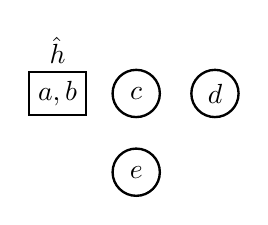
\begin{tikzpicture}
        % Singletons
        \def \cx{1}     \def \cy{0}
        \def \dx{2}     \def \dy{0}
        \def \ex{1}     \def \ey{-1}
        \def \hx{0}     \def \hy{0}

        \node[rectangle, draw, line width=0.3mm] at (\hx, \hy) {$a,b$};
        \node at (0, 0.55) {$\hat{h}$};
        \draw[line width=0.3mm] (\cx, \cy) circle (0.3) node[anchor=center]{$c$};
        \draw[line width=0.3mm] (\dx, \dy) circle (0.3) node[anchor=center]{$d$};
        \draw[line width=0.3mm] (\ex, \ey) circle (0.3) node[anchor=center]{$e$};

        % Attacks
        \DrawAttackHorizontal{R}{\hx+0.1}{\hy}{\cx}{\cy}
        \DrawSelfAttackRightSingleton{\cx}{\cy}
        \DrawAttackHorizontal{R}{\cx}{\cy}{\dx}{\dy}
        \DrawAttackVertical{D}{\cx}{\cy}{\ex}{\ey}
        \DrawAttackDiagonal{PB}{\dx}{\dy}{\ex}{\ey}
    \end{tikzpicture}
    \caption{\ac{AF} $\hat{G}$ clustered}
    \label{af:backgroundSATExample1}
\end{figure}

\paragraph{For-OR:} To concatinate all the singletons of the AF $\hat{G}$, we can use the following notation:

$$
\bigvee_{a \in \hat{G}_{\!S\!I\!N\!G\!L\!E}} a = c \lor d \lor e
$$

\paragraph{For-AND:} To concatinate all the singletons of the AF $\hat{G}$, we can use the following notation:

$$
\bigwedge_{a \in \hat{G}_{\!S\!I\!N\!G\!L\!E}} a = c \land d \land e
$$

\paragraph{For-Attacks: } To iterate over the attacks $\hat{R}$ we can extract it from the AF as tuple and address the attacker $a$ and defender $b$:

$$
\bigwedge_{(a, b) \in \hat{R}, a\in \hat{G}_{\!S\!I\!N\!G\!L\!E}} \big( a \lor b \big) = (c \lor c) \land
(c \lor d) \land (c \lor e) \land (e \lor d) \land (d \lor e)
$$

%\textit{TODO: Where and how do we use SAT-Solvers in the research}


\chapter{Algorithm to obtain Faithful Clustering}
In this chapter we have a closer look at the algorithms we designed and how they work. We provide an explanation, accompanied with an example and pseudo-code.
In \cref{sec:ConcretizingSingletons} we explain, the concretization of a clustered argument. Next, in \cref{sec:ComputationOfConcretizerList} we explain how the concretizer list (a list of clustered arguments which are mutated to singletons) is computed. The approach to compute faithful clustered AFs is described in \cref{sec:AlgorithmicApproachToComputeFaifthulClusterings}. And finally we state the heuristics and refinements in \cref{sec:HeuristicsAndRefinements}.

\textit{TODO: Update when adding sections}

\section{Concretizing Singletons}
\label{sec:ConcretizingSingletons}
When operating on clustered AFs, a crucial mutation is to extract clustered arguments from a cluster and transform it to a singleton. This is called concretizing. When clustering singletons, the cluster inherits the attacks of the argument, concretizing is the inverse operation. This means, that it needs to revert the changes done by the clustering.
Concretizing a list of arguments is done iteratively by duplicating the abstract AF $\hat{F}$ to create a new AF $\hat{F}'$ and transforming it. The transformation is guided by five steps considering the unchanged abstract AF $\hat{F}$ and the concrete AF $F$. To improve the understanding of each step, we accompany the explanation with the example depicted in \cref{example:concretizationOfArguments}, where we concretize the arguments $a$ and $b$.

\vspace{0.3cm}

\vspace{0.3cm}
\begin{figure}[h]
    \centering
    \begin{subfigure}[b]{0.475\textwidth}
        \centering
        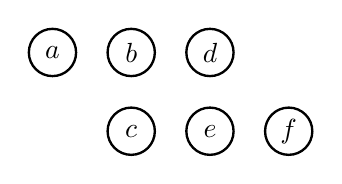
\begin{tikzpicture}
            % Singletons
                \def \ax{0}   \def \ay{0}
                \def \bx{1}   \def \by{0}
                \def \cx{1}   \def \cy{-1}
                \def \dx{2}   \def \dy{0}
                \def \ex{2}   \def \ey{-1}
                \def \fx{3}   \def \fy{-1}

                \draw[line width=0.3mm] (\ax, \ay) circle (0.3) node[anchor=center]{$a$};
                \draw[line width=0.3mm] (\bx, \by) circle (0.3) node[anchor=center]{$b$};
                \draw[line width=0.3mm] (\cx, \cy) circle (0.3) node[anchor=center]{$c$};
                \draw[line width=0.3mm] (\dx, \dy) circle (0.3) node[anchor=center]{$d$};
                \draw[line width=0.3mm] (\ex, \ey) circle (0.3) node[anchor=center]{$e$};
                \draw[line width=0.3mm] (\fx, \fy) circle (0.3) node[anchor=center]{$f$};
                % Attacks
                \DrawAttackHorizontal{L}{\bx}{\by}{\ax}{\ay}
                \DrawAttackHorizontal{L}{\dx}{\dy}{\bx}{\by}

                \DrawAttackVertical{D}{\bx}{\by}{\cx}{\cy}
                \DrawAttackVertical{U}{\ex}{\ey}{\dx}{\dy}

                \DrawAttackDiagonal{NRL}{\cx}{\cy}{\ax}{\ay}
        \end{tikzpicture}
        \caption{Concrete AF $F$}
        \label{fig:concrete_af}
    \end{subfigure}%
    \hfill
    \begin{subfigure}[b]{0.475\textwidth}
        \centering
        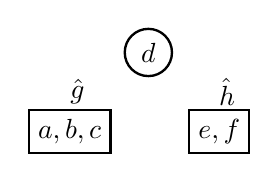
\begin{tikzpicture}
            % Singletons
            \def \dx{1}   \def \dy{0}
            \def \gx{0}   \def \gy{-1}
            \def \hx{1.9}   \def \hy{-1}

            \draw[line width=0.3mm] (\dx, \dy) circle (0.3) node[anchor=center]{$d$};
            % Cluster

            \node[rectangle, draw, line width=0.3mm] at (\gx, \gy) {$a,b,c$};
            \node at (\gx + 0.1, \gy+0.5) {$\hat{g}$};

            \node[rectangle, draw, line width=0.3mm] at (\hx, \hy) {$e,f$};
            \node at (\hx + 0.1, \hy+0.5) {$\hat{h}$};

            % Attacks
            \DrawAttackDiagonal{PRL}{\dx}{\dy}{\gx+0.1}{\gy+0.1}
            \DrawAttackDiagonal{NRL}{\hx}{\hy+0.1}{\dx}{\dy}
            \DrawSelfAttackLeftTopCluster{\gx-0.45}{\gy+0.3}
        \end{tikzpicture}
        \caption{Abstract AF $\hat{F}$}
        \label{fig:abstract_af}
    \end{subfigure}
    \caption{Concrete and abstract AF}
    \label{example:concretizationOfArguments}
\end{figure}

\paragraph{Step 1:} Each argument needing concretization is first removed from the parent cluster and added as a singleton in $\hat{F}'$.
If an argument is not part of a cluster, we ignore it.
We do not consider attacks in this step since they depend on the concrete- and abstract AFs. The resulting AF is depicted in \cref{example:algorithmConcretizeSingletonsStep1} and the pseudo-code in \cref{alg:concretizingSingletonsStep1}.


\vspace{0.3cm}
\begin{figure}[h]
    \centering
    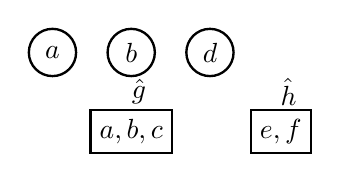
\begin{tikzpicture}
        % Singletons
        \def \ax{0}   \def \ay{0}
        \def \bx{1}   \def \by{0}
        \def \dx{2}   \def \dy{0}
        \def \gx{1}   \def \gy{-1}
        \def \hx{2.9}   \def \hy{-1}

        \draw[line width=0.3mm] (\ax, \ay) circle (0.3) node[anchor=center]{$a$};
        \draw[line width=0.3mm] (\bx, \by) circle (0.3) node[anchor=center]{$b$};
        \draw[line width=0.3mm] (\dx, \dy) circle (0.3) node[anchor=center]{$d$};
        % Cluster

        \node[rectangle, draw, line width=0.3mm] at (\gx, \gy) {$a,b,c$};
        \node at (\gx + 0.1, \gy + 0.5) {$\hat{g}$};

        \node[rectangle, draw, line width=0.3mm] at (\hx, \hy) {$e,f$};
        \node at (\hx + 0.1, \hy + 0.5) {$\hat{h}$};

        % Attacks
        \DrawAttackDiagonal{PRL}{\dx}{\dy}{\gx+0.1}{\gy+0.1}
        \DrawAttackDiagonal{NRL}{\hx}{\hy+0.1}{\dx}{\dy}
        \DrawSelfAttackLeftTopCluster{\gx-0.45}{\gy+0.3}

    \end{tikzpicture}
    \caption{Concretized AF $\hat{F}'$ after Step 1}
    \label{example:algorithmConcretizeSingletonsStep1}
\end{figure}
\vspace{-0.2cm}


\begin{algorithm}[H]
    \caption{Concretizing Singletons Pseudocode Step 1}\label{alg:concretizingSingletonsStep1}
    \begin{algorithmic}[1]
        \Require $A: AF(a_1, r_1)$ \Comment{Abstract Clustered AF}
        \Require $e: list(Arguments)$ \Comment{Concretizer List}
        \State $N$ $\gets$ $A$ \Comment{$N$ = Concretized Cluster}
        \For{$a_i$ in $e$}
            \For{$c_i$ in $A.clusters$}
                \If{$a_i$ in $c_i$}
                    \State $c_i.remove(a_i)$
                \EndIf
                \EndFor
            \State $N.addSingleton(a_i)$
        \EndFor
    \end{algorithmic}
\end{algorithm}




\paragraph{Step 2:} We add the new attacks from all concretized arguments to the remaining clusters and vice versa. We must do this after removing the arguments from the clusters because if an argument $a$ attacks argument $b$ in the concrete AF $F$, and $b$ is part of the cluster $\hat{g}$ in the abstract AF $\hat{F}$, by concretizing $b$, the attack $(a,\hat{g})$ would not be present anymore. The resulting AF $\hat{F}'$ is depicted in \cref{example:algorithmConcretizeSingletonsStep2} and the pseudo-code in \cref{alg:concretizingSingletonsStep2}


\vspace{0.3cm}
\begin{figure}[h]
    \centering
    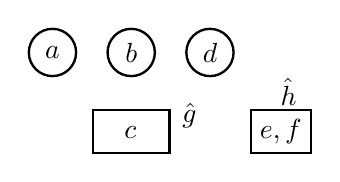
\begin{tikzpicture}
        % Singletons
        \def \ax{0}   \def \ay{0}
        \def \bx{1}   \def \by{0}
        \def \dx{2}   \def \dy{0}
        \def \gx{1}   \def \gy{-1}
        \def \hx{2.9}   \def \hy{-1}

        \draw[line width=0.3mm] (\ax, \ay) circle (0.3) node[anchor=center]{$a$};
        \draw[line width=0.3mm] (\bx, \by) circle (0.3) node[anchor=center]{$b$};
        \draw[line width=0.3mm] (\dx, \dy) circle (0.3) node[anchor=center]{$d$};
        % Cluster

        \node[rectangle, draw, line width=0.3mm] at (\gx, \gy) {$\phantom{a,} c\phantom{, b}$};
        \node at (\gx + 0.74, \gy + 0.2) {$\hat{g}$};

        \node[rectangle, draw, line width=0.3mm] at (\hx, \hy) {$e,f$};
        \node at (\hx + 0.1, \hy + 0.5) {$\hat{h}$};

        % Attacks
        \DrawAttackDiagonal{PRL}{\dx}{\dy}{\gx+0.1}{\gy+0.1}
        \DrawAttackDiagonal{NRL}{\hx}{\hy+0.1}{\dx}{\dy}
        \DrawSelfAttackLeftTopCluster{\gx-0.45}{\gy+0.3}
        \DrawAttackVertical{D}{\bx}{\by}{\gx}{\gy}
        \DrawAttackDiagonal{NRL}{\gx-0.1}{\gy+0.1}{\ax}{\ay}


    \end{tikzpicture}
    \caption{Concretized AF $\hat{F}'$ after Step 2}
    \label{example:algorithmConcretizeSingletonsStep2}
\end{figure}
\vspace{-0.2cm}



\begin{algorithm}[H]
    \caption{Concretizing Singletons Pseudocode Step 2}\label{alg:concretizingSingletonsStep2}
    \begin{algorithmic}[1]
        \Require $C: AF(a_2, r_2)$ \Comment{Concrete AF}
        \Require $e: list(Arguments)$ \Comment{Concretizer List}
        \Require $N: AF(a_3, r_3)$ \Comment{Concretized Cluster}
        \For{$e_i$ in $e$}
            \For{$att_i$ in $C[e_i].attacks$}
                \If{$att_i$ to cluster $c_i$}
                    \State $N.addAttack((e_i, c_i))$
                \EndIf
            \EndFor
            \For{$def_i$ in $C[e_i].defends$}
                \If{$def_i$ from cluster $c_i$}
                    \State $N.addAttack((c_i, e_i))$
                \EndIf
            \EndFor
        \EndFor
    \end{algorithmic}
\end{algorithm}



\paragraph{Step 3:} After adding the new attacks, we need to check which attacks from $\hat{F}$ are still present in $\hat{F}'$. If an attack does not persist through the concretization, we remove it in $\hat{F}'$. An attack is not present anymore; if we remove one of the arguments being attacked or attacked by argument $a$ from a cluster $\hat{f}$ and no other attack exists, s.t. $a$ is attacked from/attacking an argument within $\hat{f}$. Selfattacks of clusters could also change by the concretization of arguments. Therefore, we need to check the clusters from which the arguments are concretized. The resulting AF is depicted in \cref{example:algorithmConcretizeSingletonsStep3} and the pseudo-code in \cref{alg:concretizingSingletonsStep3}.


\vspace{0.3cm}
\begin{figure}[h]
    \centering
    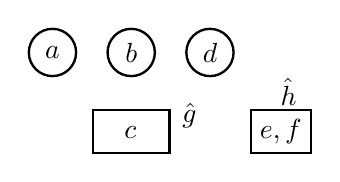
\begin{tikzpicture}
        % Singletons
        \def \ax{0}   \def \ay{0}
        \def \bx{1}   \def \by{0}
        \def \dx{2}   \def \dy{0}
        \def \gx{1}   \def \gy{-1}
        \def \hx{2.9}   \def \hy{-1}

        \draw[line width=0.3mm] (\ax, \ay) circle (0.3) node[anchor=center]{$a$};
        \draw[line width=0.3mm] (\bx, \by) circle (0.3) node[anchor=center]{$b$};
        \draw[line width=0.3mm] (\dx, \dy) circle (0.3) node[anchor=center]{$d$};
        % Cluster

        \node[rectangle, draw, line width=0.3mm] at (\gx, \gy) {$\phantom{a,} c\phantom{, b}$};
        \node at (\gx + 0.74, \gy + 0.2) {$\hat{g}$};

        \node[rectangle, draw, line width=0.3mm] at (\hx, \hy) {$e,f$};
        \node at (\hx + 0.1, \hy + 0.5) {$\hat{h}$};

        % Attacks
        \DrawAttackDiagonal{NRL}{\hx}{\hy+0.1}{\dx}{\dy}
        \DrawAttackVertical{D}{\bx}{\by}{\gx}{\gy}
        \DrawAttackDiagonal{NRL}{\gx-0.1}{\gy+0.1}{\ax}{\ay}
    \end{tikzpicture}
    \caption{Concretized AF $\hat{F}'$ after Step 3}
    \label{example:algorithmConcretizeSingletonsStep3}
\end{figure}
\vspace{-0.2cm}

\begin{algorithm}[H]
    \caption{Concretizing Singletons Pseudocode Step 3}\label{alg:concretizingSingletonsStep3}
    \begin{algorithmic}[1]
        \Require $A: AF(a_1, r_1)$ \Comment{Abstract Clustered AF}
        \Require $C: AF(a_2, r_2)$ \Comment{Concrete AF}
        \Require $N: AF(a_3, r_3)$ \Comment{Concretized Cluster}
        \For{$r_i$ in $A_{r_1}$}
            \If{$r_i.defender$ is cluster and $r_i.attacker$ is cluster}
                \If{!($r_i.attacker$ attacks any of $C[r_i].defender$)}
                    \State $N.removeAttack(r_i)$
                    \State continue
                \EndIf
            \EndIf
            \If{$r_i.defender$ is cluster}
                \If{!($r_i.attacker$ attacks any of $C[r_i].defender$)}
                    \State $N.removeAttack(r_i)$
                    \State continue
                \EndIf
            \EndIf
            \If{$r_i.attacker$ is cluster}
                \If{!($r_i.defender$ defends against any $C[r_i].attacker$)}
                    \State $N.removeAttack(r_i)$
                    \State continue
                \EndIf
            \EndIf
        \EndFor
    \end{algorithmic}
\end{algorithm}


\paragraph{Step 4:} In this step we add the new attacks between the singletons. Due to the fact, that we copied all the attacks from $\hat{F}$, we only have to take into consideration the attacks from or to the concretized singletons. So instead of iterating over all singletons of the AF $\hat{F}'$, we can limit the attack creation to the concretized singletons. The resulting AF is depicted in \cref{example:algorithmConcretizeSingletonsStep4} and the pseudo-code in \cref{alg:concretizingSingletonsStep4}.


\vspace{0.3cm}
\begin{figure}[h]
    \centering
    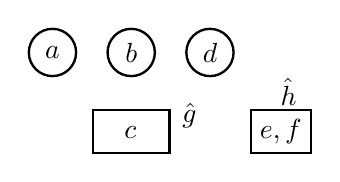
\begin{tikzpicture}
        % Singletons
        \def \ax{0}   \def \ay{0}
        \def \bx{1}   \def \by{0}
        \def \dx{2}   \def \dy{0}
        \def \gx{1}   \def \gy{-1}
        \def \hx{2.9}   \def \hy{-1}

        \draw[line width=0.3mm] (\ax, \ay) circle (0.3) node[anchor=center]{$a$};
        \draw[line width=0.3mm] (\bx, \by) circle (0.3) node[anchor=center]{$b$};
        \draw[line width=0.3mm] (\dx, \dy) circle (0.3) node[anchor=center]{$d$};
        % Cluster

        \node[rectangle, draw, line width=0.3mm] at (\gx, \gy) {$\phantom{a,} c\phantom{, b}$};
        \node at (\gx + 0.74, \gy + 0.2) {$\hat{g}$};

        \node[rectangle, draw, line width=0.3mm] at (\hx, \hy) {$e,f$};
        \node at (\hx + 0.1, \hy + 0.5) {$\hat{h}$};

        % Attacks
        \DrawAttackDiagonal{NRL}{\hx}{\hy+0.1}{\dx}{\dy}
        \DrawAttackVertical{D}{\bx}{\by}{\gx}{\gy}
        \DrawAttackDiagonal{NRL}{\gx-0.1}{\gy+0.1}{\ax}{\ay}
        \DrawAttackHorizontal{L}{\dx}{\dy}{\bx}{\by}
        \DrawAttackHorizontal{L}{\bx}{\by}{\ax}{\ay}
    \end{tikzpicture}
    \caption{Concretized AF $\hat{F}'$ after Step 4}
    \label{example:algorithmConcretizeSingletonsStep4}
\end{figure}
\vspace{-0.2cm}


\begin{algorithm}[H]
    \caption{Concretizing Singletons Pseudocode Step 4}\label{alg:concretizingSingletonsStep4}
    \begin{algorithmic}[1]
        \Require $A: AF(a_1, r_1)$ \Comment{Abstract Clustered AF}
        \Require $C: AF(a_2, r_2)$ \Comment{Concrete AF}
        \Require $e: list(Arguments)$ \Comment{Concretizer List}
        \Require $N: AF(a_3, r_3)$ \Comment{Concretized Cluster}
        \For{$e_i$ in $e$}
            \For{$a_i$ in $C[e_i].attacks$}
                \If{$a_i$ is singleton and ($e_i$, $a_i$) not in $r_2$}
                    \State $N.addAttack((e_i, a_i))$
                \EndIf
            \EndFor
            \For{$a_i$ in $C[e_i].defends$}
                \If{$a_i$ is singleton and ($a_i$, $e_i$) not in $r_2$}
                    \State $N.addAttack((a_i, e_i))$
                \EndIf
            \EndFor
        \EndFor
    \end{algorithmic}
\end{algorithm}


\paragraph{Step 5:} The last step is to clean up the argumentation framework $\hat{F}'$ by removing all empty clusters and mutating the clusters with exactly
one singleton to the mentioned singleton. The resulting AF $\hat{F}'$ is depicted in \cref{example:algorithmConcretizeSingletonsStep5} and the pseudo-code in \cref{alg:concretizingSingletonsStep5}.


\vspace{0.3cm}
\begin{figure}[h!]
    \centering
    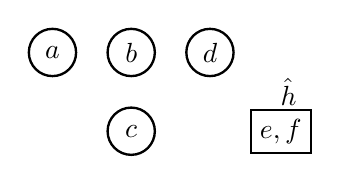
\begin{tikzpicture}
        % Singletons
        \def \ax{0}   \def \ay{0}
        \def \bx{1}   \def \by{0}
        \def \dx{2}   \def \dy{0}
        \def \cx{1}   \def \cy{-1}
        \def \hx{2.9}   \def \hy{-1}

        \draw[line width=0.3mm] (\ax, \ay) circle (0.3) node[anchor=center]{$a$};
        \draw[line width=0.3mm] (\bx, \by) circle (0.3) node[anchor=center]{$b$};
        \draw[line width=0.3mm] (\cx, \cy) circle (0.3) node[anchor=center]{$c$};
        \draw[line width=0.3mm] (\dx, \dy) circle (0.3) node[anchor=center]{$d$};
        % Cluster
        \node[rectangle, draw, line width=0.3mm] at (\hx, \hy) {$e,f$};
        \node at (\hx + 0.1, \hy + 0.5) {$\hat{h}$};

        % Attacks
        \DrawAttackDiagonal{NRL}{\hx}{\hy+0.1}{\dx}{\dy}
        \DrawAttackVertical{D}{\bx}{\by}{\cx}{\cy}
        \DrawAttackDiagonal{NRL}{\cx}{\cy}{\ax}{\ay}
        \DrawAttackHorizontal{L}{\dx}{\dy}{\bx}{\by}
        \DrawAttackHorizontal{L}{\bx}{\by}{\ax}{\ay}
    \end{tikzpicture}
    \caption{Concretized AF $\hat{F}'$ after Step 5}
    \label{example:algorithmConcretizeSingletonsStep5}
\end{figure}
\vspace{-0.2cm}

\begin{algorithm}[H]
    \caption{Concretizing Singletons Pseudocode Step 5}\label{alg:concretizingSingletonsStep5}
    \begin{algorithmic}[1]
        \Require $A: AF(a_1, r_1)$ \Comment{Abstract Clustered AF}
        \Require $C: AF(a_2, r_2)$ \Comment{Concrete AF}
        \Require $e: list(Arguments)$ \Comment{Concretizer List}
        \Require $N: AF(a_3, r_3)$ \Comment{Concretized Cluster}
        \For{$c_i$ in $N.clusters$}
            \If{$c_i.argAmount == 1$}
                \State $c_i \gets Singleton$
            \ElsIf{$c_i.argAmount == 0$}
                \State $N.remove(c_i)$
            \EndIf
        \EndFor
    \end{algorithmic}
\end{algorithm}


\newpage
\section{Computation of Concretizer List}
\label{sec:ComputationOfConcretizerList}
% Why do we need the algorithm
When talking about clustering AFs, faithfulness is an important property. If an AF is spurious, we found atleast one semantics extension, which cannot be mapped to a concrete extension. Based on the spurious extensions, we try to mutate the clustered AF, to obtain faithfulness. This mutation is realized through the concretizer list.

% What is concretizer list
The concretizer list is a list of sets of clustered arguments. Each set is a unique combination of arguments, which are being concretized to find a faithful AF. All the sets of the concretizer list are attempted iteratively, where the order is dependend on the size of the set. We use a heuristicical approach, putting the main focus on local changes. Here we operate directly on the arguments and its attackers which make a set spurious, instead of applying global changes to the AF. Further, a minimal deviation of the abstract AF is usually desired, so small concretizer sets are checked first.

% Input: spurious set
The input to the computation of the concretizer list is a set of the arguments of all the spurious semantics extensions. The size and computation intensity of the concretizer list is highly dependent on the amount of attacks, each argument of the input set and its neighbours with depth 2 have. This is also the critical part of the faithful AF computation and makes some AFs infeasible to solve.

% Example base
Let us have a look at an example to demonstrate how the concretizer list is computed. The concrete AF $G$ is defined in \cref{af:algorithmConcretizer1} and the according abstract AF $\hat{G}$ in \cref{af:algorithmConcretizer2}.


\vspace{0.3cm}
\begin{figure}[h]
\begin{minipage}{.5\textwidth}
    \centering
    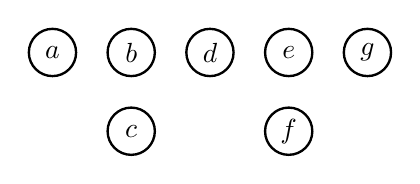
\begin{tikzpicture}
        % Singletons
        \def \ax{0}   \def \ay{0}
        \def \bx{1}   \def \by{0}
        \def \cx{1}   \def \cy{-1}
        \def \dx{2}   \def \dy{0}
        \def \ex{3}   \def \ey{0}
        \def \fx{3}   \def \fy{-1}
        \def \gx{4}   \def \gy{0}

        \draw[line width=0.3mm] (\ax, \ay) circle (0.3) node[anchor=center]{$a$};
        \draw[line width=0.3mm] (\bx, \by) circle (0.3) node[anchor=center]{$b$};
        \draw[line width=0.3mm] (\cx, \cy) circle (0.3) node[anchor=center]{$c$};
        \draw[line width=0.3mm] (\dx, \dy) circle (0.3) node[anchor=center]{$d$};
        \draw[line width=0.3mm] (\ex, \ey) circle (0.3) node[anchor=center]{$e$};
        \draw[line width=0.3mm] (\fx, \fy) circle (0.3) node[anchor=center]{$f$};
        \draw[line width=0.3mm] (\gx, \gy) circle (0.3) node[anchor=center]{$g$};

        % Attacks
        \DrawSelfAttackLeftSingleton{\ax}{\ay}
        \DrawAttackHorizontal{B}{\bx}{\by}{\ax}{\ay}
        \DrawAttackHorizontal{R}{\bx}{\by}{\dx}{\dy}
        \DrawAttackHorizontal{B}{\ex}{\ey}{\dx}{\dy}
        \DrawAttackHorizontal{R}{\ex}{\ey}{\gx}{\gy}
        \DrawAttackVertical{B}{\bx}{\by}{\cx}{\cy}
        \DrawAttackVertical{D}{\ex}{\ey}{\fx}{\fy}
        \DrawAttackDiagonal{PLR}{\fx}{\fy}{\gx}{\gy}
    \end{tikzpicture}
    \subcaption{Concrete AF $G$}
    \label{af:algorithmConcretizer1}
\end{minipage}%
\begin{minipage}{.5\textwidth}
    \centering
    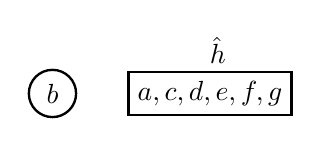
\begin{tikzpicture}
        % Singletons
        \def \bx{0}   \def \by{0}
        \def \hx{2}   \def \hy{0}

        \draw[line width=0.3mm] (\bx, \by) circle (0.3) node[anchor=center]{$b$};

        % Cluster
        \node[rectangle, draw, line width=0.3mm] at (\hx, \hy) {$a, c, d, e, f, g$};
        \node at (\hx + 0.1, \hy + 0.55) {$\hat{h}$};
        % Attacks
        \DrawAttackHorizontal{B}{\hx-0.85}{\hy}{\bx}{\by}
        \DrawSelfAttackRightTopCluster{\hx+1}{\hy+0.29}

    \end{tikzpicture}
    \subcaption{Abstract AF $\hat{G}$}
    \label{af:algorithmConcretizer2}
\end{minipage}
\caption{Concrete and abstract AF}
\label{fig:comparison}
\end{figure}
\vspace{0.3cm}

If we have a look at the stable extensions of the concrete AF $G$, e.g.\ 
$\mathtt{stb=}\bigl\{\{b, c\}\bigl\}$ and at the abstractly stable extensions of the abstract AF $\hat{G}$, e.g.\ 
$\mathtt{\hat{stb}=}\bigl\{\{b, \hat{h}\}, \{\hat{h}\}, \{b\}\bigl\}$, we can see that the abstractly stable extensions $\{\hat{h}\}$ and $\{b\}$ are spurious. The input to the concretizer list computation is a collection of the arguments of all the spurious sets, which in this case is $\{b, \hat{h}\}$.

% Filter Cluster out of spurious set, because we cant concretize cluster
The first step is to filter out the clusters of the input, since clusters are not present in the concrete AF and therefore do not attack any singletons and are not being attacked. So we reduce the concretizer list from $\{b, \hat{h}\}$ to $\{b\}$. The pseudo-code is listed in \cref{alg:concretizerListPrefiltering}.

\begin{algorithm}[H]
    \caption{Computation of Concretizer list Algorithm: Prefiltering}\label{alg:concretizerListPrefiltering}
    \begin{algorithmic}[1]
        \Require $\hat{G}: AF(a_2, r_2)$ \Comment{Abstract AF}
        \Require $s: list(Arguments)$ \Comment{spurious arguments}
        \For{$s_i$ in $s$}
            \If{$s_i$ in $\hat{G}$ is cluster}
                \State $s$.remove($s_i$)
            \EndIf
        \EndFor
    \end{algorithmic}
\end{algorithm}

% Get combination as attacker depth 2
% Get combination as defender depth 2
Next, we have a look at the neighbouring arguments of the current concretizer list.  Neighbours in this context are arguments which attack, or are being attacked by an argument. The depth defines how many arguments are between the attacks. A depth of $0$ is the actual argument, a depth of $1$ represents the direct attacker of the argument and the direct arguments, which are being attacked by the argument. A depth $2$ argument is an argument, which has some attack relation (e.g.\ attacks the argument or is attacked by the argument) with a depth $1$ argument.

We used a search depth of $2$ in our implementation. So when having a look at our example, we take the defender of depth $1$ and $2$, in \cref{af:algorithmConcretizer3} depicted in yellow and the attacker with the same depth, depicted in blue. The pseudo-code of this procedure is listed in \cref{alg:concretizerListNeighbours}. Some arguments can have multiple depths (e.g.\ argument $c$. It is a direct attacker of the argument $b$ with depth $0$, but also a direct attacker of the argument $c$ with depth $1$), than the lower depth is chosen as the representative.

%Depth 2 Attacker
\vspace{0.1cm}
\begin{figure}[h!]
    \centering
    \begin{tikzpicture}
        % Singletons
        \def \ax{0}   \def \ay{0}
        \def \bx{1}   \def \by{0}
        \def \cx{1}   \def \cy{-1}
        \def \dx{2}   \def \dy{0}
        \def \ex{3}   \def \ey{0}
        \def \fx{3}   \def \fy{-1}
        \def \gx{4}   \def \gy{0}

        \draw[line width=0.3mm] (\ax, \ay) circle (0.3) node[anchor=center]{$a$};
        \draw[cYellow] (\ax,\ay) circle (0.4);
        \node[text=cYellow] at (\ax+0.33, \ay+0.45) {\footnotesize 1};

        \draw[line width=0.3mm] (\bx, \by) circle (0.3) node[anchor=center]{$b$};
        \draw[cRed] (\bx,\by) circle (0.4);
        \node[text=cRed] at (\bx+0.33, \by+0.45) {\footnotesize 0};

        \draw[line width=0.3mm] (\cx, \cy) circle (0.3) node[anchor=center]{$c$};
        \draw[cYellow] (\cx,\cy) circle (0.4);
        \node[text=cYellow] at (\cx+0.55, \cy) {\footnotesize 1};

        \draw[line width=0.3mm] (\dx, \dy) circle (0.3) node[anchor=center]{$d$};
        \draw[cBlue] (\dx,\dy) circle (0.4);
        \node[text=cBlue] at (\dx+0.33, \dy+0.45) {\footnotesize 1};

        \draw[line width=0.3mm] (\ex, \ey) circle (0.3) node[anchor=center]{$e$};
        \draw[cBlue] (\ex,\ey) circle (0.4);
        \node[text=cBlue] at (\ex+0.33, \ey+0.45) {\footnotesize 2};

        \draw[line width=0.3mm] (\fx, \fy) circle (0.3) node[anchor=center]{$f$};
        \node at (\fx+0.45, \fy) {\footnotesize 3};

        \draw[line width=0.3mm] (\gx, \gy) circle (0.3) node[anchor=center]{$g$};
        \node at (\gx+0.33, \gy+0.45) {\footnotesize 3};

        % Attacks
        \DrawSelfAttackLeftSingleton{\ax}{\ay}
        \DrawSelfAttackLeftSingleton{\cx}{\cy}
        \DrawAttackHorizontal{B}{\bx}{\by}{\ax}{\ay}
        \DrawAttackHorizontal{R}{\bx}{\by}{\dx}{\dy}
        \DrawAttackHorizontal{B}{\ex}{\ey}{\dx}{\dy}
        \DrawAttackHorizontal{R}{\ex}{\ey}{\gx}{\gy}
        \DrawAttackVertical{B}{\bx}{\by}{\cx}{\cy}
        \DrawAttackVertical{D}{\ex}{\ey}{\fx}{\fy}
        \DrawAttackDiagonal{PLR}{\fx}{\fy}{\gx}{\gy}
    \end{tikzpicture}
    \caption{Singletons depth with $b$ as viewpoint}
    \label{af:algorithmConcretizer3}
\end{figure}
\vspace{-0.2cm}

\begin{algorithm}
    \caption{Computation of Concretizer list Algorithm: Neighbours}\label{alg:concretizerListNeighbours}
    \begin{algorithmic}[1]
        \Require $G: AF(a_1, r_1)$ \Comment{Concrete AF}
        \Require $s: list(Arguments)$ \Comment{Working List}
        \State $N$ $\gets$ $[]$ \Comment{$N$ = list of neighbours}
        \For{$s_i$ in $s$} \Comment{Get neighbours}
            \For{$n(1)_i$ neighbour of $s_i$} \Comment{depth 1 attacker}
                \For{$n(2)_i$ neighbour of $n(1)_i$} \Comment{depth 2 attacker}
                    \State $N.append(n(1)_i$)
                    \State $N.append(n(2)_i$)
                \EndFor
            \EndFor
        \EndFor
    \end{algorithmic}
\end{algorithm}


Now the concretizer list is expanded with all the possible combinations of the neighbours. The neighbours of the current example are $\{a, c, d, e\}$. When building the combinations, we create the table defined in \cref{table:algorithmConcretizer1}.

\begin{table}[htb]
    \centering
    \begin{tabular}{ |c|c|c|c| }
     \hline
     size $1$ & size $2$ & size $3$ & size $4$\\
     \hline
     \hline
     $\{a\}$ & $\{a, c\}$ & $\{a, c, d\}$ &$\{a, c, d, e\}$ \\
     \hline
     $\{c\}$ & $\{a, d\}$ & $\{a, c, e\}$ & \\
     \hline
     $\{d\}$ & $\{a, e\}$ & $\{a, d, e\}$ & \\
     \hline
     $\{e\}$ & $\{c, d\}$ & $\{c, d, e\}$ & \\
     \hline
       & $\{c, e\}$ &  & \\
     \hline
       & $\{d, e\}$ &  & \\
     \hline
    \end{tabular}
\caption{Combinations of $\{a, c, d, e\}$}
\label{table:algorithmConcretizer1}

\end{table}

The combination table grows exponentially to the base of 2. Therefore, the size of the neighbours is crucial. If we have too many neighbours, the computation would need too much memory and turns infeasible to compute.

% Add concretizer list defined by the user
% deduplicate
If the user has provided arguments which have to be concretized as program argument, we add them to each combination set. After adding them, we filter for duplicates to keep the concretizer list size to a minimum.

% Filter singletons which are not in cluster, because cant concretize singletons
% deduplicate
Next, we need to filter out the arguments, which are not in clusters, since singletons are already concrete. This filtering could lead to some duplicates again, which we need to remove once again to minimize the memory consumption and reduce the amount of faitfhul checks.

Finally, we sort the list by the set size and return it. In the current example we would return the whole table, because no concretizer arguments were provided by the user. So the concretizer list would be
$\bigl\{\{a\}$
$\{b\}$
$\{c\}$
$\{d\}$
$\{a, c\}$
$\{a, d\}$
$\{a, e\}$
$\{c, d\}$
$\{c, e\}$
$\{d, e\}$
$\{a, c, d\}$
$\{a, c, e\}$
$\{a, d, e\}$
$\{c, d, e\}$
$\{a, c, d, e\}\bigl\}$. The pseudo-code for the last step is stated in \cref{alg:concretizerListCombinationAndCleanup}.


\begin{algorithm}
    \caption{Computation of Concretizer list Algorithm: Combinations and Cleanup}\label{alg:concretizerListCombinationAndCleanup}
    \begin{algorithmic}[1]
        \Require $G: AF(a_1, r_1)$ \Comment{Concrete AF}
        \Require $\hat{G}: AF(a_2, r_2)$ \Comment{Abstract AF}
        \Require $s: list(Arguments)$ \Comment{Working List}
        \Require $ca: list(Arguments)$ \Comment{Concretize arguments parameter}

        \State $C \gets$ combinations of N with $range(1, len(N)-1)$ \Comment{Combination List}

        \For{$ca_i$ in $ca$} \Comment{Parameter Arguments to be concretized}
            \For{$c_i$ in $C$}
                \State $c_i.append(ca_i)$
            \EndFor
        \EndFor
        \State $C.deduplicate()$

        \For{$s_i$ in $C$} \Comment{Remove clusters}
            \For{$a_i$ in $s_i$}
                \If{$\hat{G}[a_i]$ is cluster}
                    \State $s_i.remove(a_i)$
                \EndIf
            \EndFor
        \EndFor
        \State \Return $s.sortBySize()$
    \end{algorithmic}
\end{algorithm}

When concretizing the list, we find a set which leads to a faithful AF: $\{a, c, d\}$ depicted in \cref{af:algorithmConcretizer4}.

\begin{figure}[H]
    \centering
    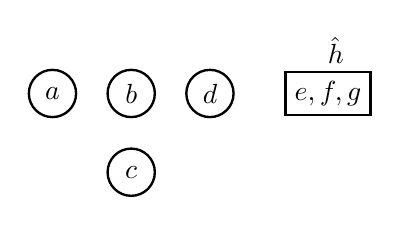
\begin{tikzpicture}
        % Singletons
        \def \ax{0}   \def \ay{0}
        \def \bx{1}   \def \by{0}
        \def \cx{1}   \def \cy{-1}
        \def \dx{2}   \def \dy{0}
        \def \hx{3.5}   \def \hy{0}

        \draw[line width=0.3mm] (\ax, \ay) circle (0.3) node[anchor=center]{$a$};
        \draw[line width=0.3mm] (\bx, \by) circle (0.3) node[anchor=center]{$b$};
        \draw[line width=0.3mm] (\cx, \cy) circle (0.3) node[anchor=center]{$c$};
        \draw[line width=0.3mm] (\dx, \dy) circle (0.3) node[anchor=center]{$d$};

        % Cluster
        \node[rectangle, draw, line width=0.3mm] at (\hx, \hy) {$e, f, g$};
        \node at (\hx + 0.1, \hy + 0.55) {$\hat{h}$};
        % Attacks
        \DrawAttackHorizontal{B}{\hx-0.3}{\hy}{\dx}{\dy}
        \DrawAttackHorizontal{B}{\bx}{\by}{\ax}{\ay}
        \DrawAttackHorizontal{R}{\bx}{\by}{\dx}{\dy}
        \DrawAttackVertical{B}{\bx}{\by}{\cx}{\cy}
        \DrawSelfAttackRightTopCluster{\hx+0.45}{\hy+0.29}
        \DrawSelfAttackLeftSingleton{\ax}{\ay}

    \end{tikzpicture}
    \caption{Faithful AF $\hat{G}'$}
    \label{af:algorithmConcretizer4}
\end{figure}



\newpage

\section{Encodings}
\label{sec:Encodings}
We previously defined the semantics in mathematical notation. But since we use SAT-Solving to obtain semantics sets, we have to bring them into a Boolean form. We will accompany each Boolean formula of the specific semantics with an example AF, the according Boolean resolution and the satisfiable models.


\paragraph{Conflict-Free} A set of arguments is (abstractly) conflict-free, if each Boolean (representing an argument) of the set is \emph{true} and the formula defined in \cref{def:booleanFormulaConflictFree} is satisfiable. For conflict-freeness, the expression is always satisfiable with the empty set (i.e.\ every Boolean is set to \emph{false}) and is therefore part of the conflict-free sets. Every other model that satisfies the formula is also part of the conflict-free set.

\begin{definition}
    Let $G=(A,R)$ be an AF. Then all the satisfiable models of the following formula are (abstractly) conflict-free.
    \begin{center}
        \[ \hat{cf}(G)=
        \bigwedge_{a \in A_{\!S\!I\!N\!G\!L\!E}} \bigl( \bigwedge_{b:(b,a)\in R, b \in A_{\!S\!I\!N\!G\!L\!E}} \lnot \bigl( a \wedge b \bigl) \bigl)
        \]
    \end{center}
    \label{def:booleanFormulaConflictFree}
\end{definition}


\begin{example}
    Let us have a look at an example and define the AF $G=(A,R)$ to be the AF depicted in \cref{af:algorithmEncodingsConflictFree}. Where the arguments are $A=\{a, b, c, d\}$ and the attacks $R=\big\{ (a,a), (a,b), (b,c), (d,a), (d,b), (d,c)\big\}$.

    \begin{figure}[H]
        \centering
        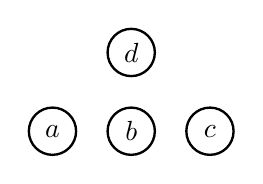
\begin{tikzpicture}
            % Singletons
            \def \ax{0}   \def \ay{-1}
            \def \bx{1}   \def \by{-1}
            \def \cx{2}   \def \cy{-1}
            \def \dx{1}   \def \dy{0}

            \draw[line width=0.3mm] (\ax, \ay) circle (0.3) node[anchor=center]{$a$};
            \draw[line width=0.3mm] (\bx, \by) circle (0.3) node[anchor=center]{$b$};
            \draw[line width=0.3mm] (\cx, \cy) circle (0.3) node[anchor=center]{$c$};
            \draw[line width=0.3mm] (\dx, \dy) circle (0.3) node[anchor=center]{$d$};

            % Attacks
            \DrawAttackHorizontal{R}{\ax}{\ay}{\bx}{\by}
            \DrawAttackHorizontal{R}{\bx}{\by}{\cx}{\cy}
            \DrawSelfAttackLeftSingleton{\ax}{\ay}
            \DrawAttackDiagonal{PRL}{\dx}{\dy}{\ax}{\ay}
            \DrawAttackDiagonal{NLR}{\dx}{\dy}{\cx}{\cy}
            \DrawAttackVertical{D}{\dx}{\dy}{\bx}{\by}
        \end{tikzpicture}
        \caption{Concrete AF $G$}
        \label{af:algorithmEncodingsConflictFree}
    \end{figure}

By applying the conflict-free formula to the AF $G$, we obtain the Boolean resolution.

\begin{align*}
    \psi =
    \lnot(b \land a)  \land
    \lnot(b \land d)  \land
    & \lnot(a \land d)  \land
    \lnot(a \land a)  \land
    \\
    & \lnot(c \land b)  \land
    \lnot(c \land d)
\end{align*}

The satisfiable models of $\psi$, and thus, the (abstractly) conflict-free sets of the AF $G$ are $\bigl\{$ $\{\}$ $\{b\}$, $\{c\}$, $\{d\}$ $\bigl\}$.
\end{example}


\paragraph{Admissible} Every satisfiable model of \cref{def:booleanFormulaAdmissible} is an (abstractly) admissible set. For admissibility, the empty set does always satisfy the formula and therefore is always part of the admissible sets. Besides the empty set, every model which satisfies the formula is also part of the admissible sets.

\begin{definition}
    Let $G=(A,R)$ be an AF. Then all the satisfiable models of the following formula are (abstractly) admissible.
    \begin{center}
        \[ \hat{adm}(G)=
        \hat{cf}(G) \land  \bigwedge_{a \in A_{\!S\!I\!N\!G\!L\!E}} \big( a \rightarrow \bigwedge_{b:(b,a) \in R} \big( \bigvee_{c:(c,b) \in R} c\big) \big)
        \]
    \end{center}
    \label{def:booleanFormulaAdmissible}
\end{definition}


\begin{example}
    Let us have a look at an example and define the AF $G=(A,R)$ to be the AF depicted in \cref{af:algorithmEncodingsAdmissible}. Where the arguments are $A=\{a, b, c, d, e\}$ and the attacks $R=\big\{ (a,a), (a,b), (b,c), (d,a), (d,b), (d,d), (d, e), (e, d)\big\}$.

    \begin{figure}[H]
        \centering
        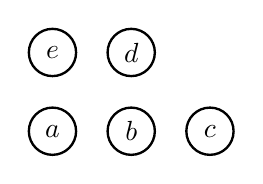
\begin{tikzpicture}
            % Singletons
            \def \ax{0}   \def \ay{-1}
            \def \bx{1}   \def \by{-1}
            \def \cx{2}   \def \cy{-1}
            \def \dx{1}   \def \dy{0}
            \def \ex{0}   \def \ey{0}

            \draw[line width=0.3mm] (\ax, \ay) circle (0.3) node[anchor=center]{$a$};
            \draw[line width=0.3mm] (\bx, \by) circle (0.3) node[anchor=center]{$b$};
            \draw[line width=0.3mm] (\cx, \cy) circle (0.3) node[anchor=center]{$c$};
            \draw[line width=0.3mm] (\dx, \dy) circle (0.3) node[anchor=center]{$d$};
            \draw[line width=0.3mm] (\ex, \ey) circle (0.3) node[anchor=center]{$e$};

            % Attacks
            \DrawAttackHorizontal{R}{\ax}{\ay}{\bx}{\by}
            \DrawAttackHorizontal{R}{\bx}{\by}{\cx}{\cy}
            \DrawAttackHorizontal{B}{\dx}{\dy}{\ex}{\ey}
            \DrawSelfAttackLeftSingleton{\ax}{\ay}
            \DrawSelfAttackRightSingleton{\dx}{\dy}
            \DrawAttackDiagonal{PRL}{\dx}{\dy}{\ax}{\ay}
            \DrawAttackVertical{D}{\dx}{\dy}{\bx}{\by}
        \end{tikzpicture}
        \caption{Concrete AF $G$}
        \label{af:algorithmEncodingsAdmissible}
    \end{figure}

By applying the admissible formula defined in \cref{def:booleanFormulaAdmissible} to the AF $G$, we obtain the Boolean resolution.

\begin{align*}
    \psi = \big(
    \lnot (a \land a)
    & \land \lnot (a \land d) \land \lnot (b \land d) \land \lnot (b \land c) \land \lnot (b \land d) \land \lnot (c \land b) \land \lnot (d \land e) \\
    & \land \lnot (d \land d) \land \lnot (e \land d) \big) \\
    & \land \bigl( a \rightarrow ((a \lor d) \land (e \lor d)) \land \bigl( b \rightarrow ((a \lor d) \land (b) \land (e \lor d)) \bigl) \bigl)\\
    & \land \bigl( c \rightarrow (a \lor c \lor d) \bigl) \land \bigl( d \rightarrow (d) \land (e \lor d) \bigl) \land \bigl( e \rightarrow (e \lor d) \bigl)
\end{align*}

The satisfiable models of $\psi$, and thus, the (abstractly) admissible sets of the AF $G$ are $\big\{ \{\},$ $\{e\},$ $\{c, e\}$ $\big\}$.
\end{example}



\paragraph{Stable} Every satisfiable model of \cref{def:booleanFormulaStable} is an (abstractly) stable extension. In contrast to conflict-free and admissible, the empty set does not satisfy the expression and therefore is never part of the stable extensions.

\begin{definition}
    Let $G=(A,R)$ be an AF. Then all the satisfiable of the following formula are (abstractly) stable extensions.
    \begin{center}
        \[ \hat{stb}(G)=
        \hat{cf}(G) \land \bigwedge_{a \in A} \big( a \bigvee_{b:(b,a)\in R} b\big) \land \bigwedge_{a \in A} \big( \big(  a \bigwedge_{b:(b,a) \in R} \lnot b\big)  \rightarrow \big( \bigwedge_{c:(a,c), c \in A_{\!S\!I\!N\!G\!L\!E}} \lnot c\big) \big)
        \]
    \end{center}
    \label{def:booleanFormulaStable}
\end{definition}


\begin{example}
    Let us have a look at an example and define the AF $G=(A,R)$ to be the AF depicted in \cref{af:algorithmEncodingsStable}. Where the arguments are $A=\{a, b, c, d\}$ and the attacks $R=\big\{ (a,a), (a,b), (a,d), (b,a), (b,d), (c,b), (d,a)\big\}$.

    \begin{figure}[H]
        \centering
        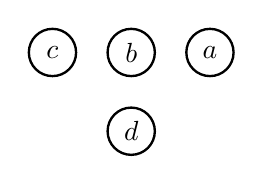
\begin{tikzpicture}
            % Singletons
            \def \ax{2}   \def \ay{0}
            \def \bx{1}   \def \by{0}
            \def \cx{0}   \def \cy{0}
            \def \dx{1}   \def \dy{-1}

            \draw[line width=0.3mm] (\ax, \ay) circle (0.3) node[anchor=center]{$a$};
            \draw[line width=0.3mm] (\bx, \by) circle (0.3) node[anchor=center]{$b$};
            \draw[line width=0.3mm] (\cx, \cy) circle (0.3) node[anchor=center]{$c$};
            \draw[line width=0.3mm] (\dx, \dy) circle (0.3) node[anchor=center]{$d$};

            % Attacks
            \DrawSelfAttackRightSingleton{\ax}{\ay}
            \DrawAttackHorizontal{R}{\cx}{\cy}{\bx}{\by}
            \DrawAttackHorizontal{B}{\ax}{\ay}{\bx}{\by}
            \DrawAttackVertical{D}{\bx}{\by}{\dx}{\dy}
            \DrawAttackDiagonal{PLR}{\dx}{\dy}{\ax}{\ay}
        \end{tikzpicture}
        \caption{Concrete AF $G$}
        \label{af:algorithmEncodingsStable}
    \end{figure}

If we apply the encoded formula for the stable semantics defined in \cref{def:booleanFormulaStable} to the AF $G$, we obtain the following Boolean resolution.

\begin{align*}
    \psi = \bigl( (\lnot (a \land a)) \land (\lnot (a \land b)) &\land (\lnot (a \land d)) \land (\lnot (b \land a)) \land (\lnot (b \land c)) \land (\lnot (d \land b)) \land (\lnot (d \land a)) \bigl) \\
    &\land \bigl( (a \lor a \lor b \lor d) \land (a \lor b \lor c) \land (a \lor b \lor d) \bigl) \\
    &\land \bigl( ((a \land \lnot a \land \lnot b \land \lnot d) \rightarrow (\lnot a \land \lnot b \land \lnot d)\bigl)\\
    &\land \bigl((b \land \lnot a \land \lnot c) \rightarrow \lnot a \land \lnot d) \land ((d \land \lnot b \land \lnot a) \rightarrow \lnot a)\bigl)
\end{align*}


The satisfiable models of $\psi$, and therefore, the stable extensions of the AF $G$ is $\bigl\{ \{c, d\}\bigl\}$.
\end{example}

\newpage

\section{Algorithmic Approach to Compute Faifthul Clusterings}
\label{sec:AlgorithmicApproachToComputeFaifthulClusterings}
When clustering AFs, information gets lost. If crucial information is abstracted in a way, s.t. we can draw erroneous conclusions, we have a spurious AF. Spurious abstract AFs do not represent the according concrete AFs. Thus, we need to mutate the clustered AF, that only correct solutions can be drawen, which we then call faithful.

\section{Heuristics and Refinements}
\label{sec:HeuristicsAndRefinements}
\textit{TODO: Define every Heuristic and refinement we used for each semantic}


\chapter{Implementations}


\section{Creating AFs}
\textit{TODO: Explain AF creation algorithms (Random + Grid-Based)}



\section{BFS and DFS Approach}
\textit{TODO: BFS and DFS approach in current research + when BFS is better than DFS}

\section{Generating Semantic Sets}
\textit{TODO: Semantic sets generation algorithm}

\section{Faithful/Spurious Determination}
\textit{TODO: Determine faithful/spurious algorithm}


REUSE THIS SOMEWHERE:

We encoded the semantics rules into Boolean formula and used the SAT-Solver to evaluate them. To cover all possibilities of AFs, we generalized the formulas and used short notation to concatinate the variables. Let us have a look at a concrete example with an abstract clustered AF $\mathtt{\hat{G}=(\hat{A}, \hat{R})}$ defined in \cref{af:backgroundSATExample1}.



\begin{figure}[h]
    \centering
    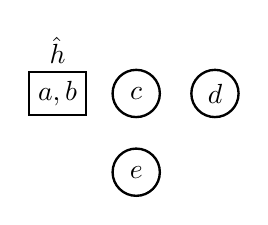
\begin{tikzpicture}
        % Singletons
        \def \cx{1}     \def \cy{0}
        \def \dx{2}     \def \dy{0}
        \def \ex{1}     \def \ey{-1}
        \def \hx{0}     \def \hy{0}

        \node[rectangle, draw, line width=0.3mm] at (\hx, \hy) {$a,b$};
        \node at (0, 0.55) {$\hat{h}$};
        \draw[line width=0.3mm] (\cx, \cy) circle (0.3) node[anchor=center]{$c$};
        \draw[line width=0.3mm] (\dx, \dy) circle (0.3) node[anchor=center]{$d$};
        \draw[line width=0.3mm] (\ex, \ey) circle (0.3) node[anchor=center]{$e$};

        % Attacks
        \DrawAttackHorizontal{R}{\hx+0.1}{\hy}{\cx}{\cy}
        \DrawSelfAttackRightSingleton{\cx}{\cy}
        \DrawAttackHorizontal{R}{\cx}{\cy}{\dx}{\dy}
        \DrawAttackVertical{D}{\cx}{\cy}{\ex}{\ey}
        \DrawAttackDiagonal{PB}{\dx}{\dy}{\ex}{\ey}
    \end{tikzpicture}
    \caption{Abstract AF $\mathtt{\hat{G}}$}
    \label{af:backgroundSATExample1}
\end{figure}


\paragraph{For-OR} To concatinate all the singletons of the AF $\hat{G}$, we can use the following notation:

$$
\bigvee_{a \in \hat{G}_{\!S\!I\!N\!G\!L\!E}} a = c \lor d \lor e
$$

\paragraph{For-AND} To concatinate all the singletons of the AF $\hat{G}$, we can use the following notation:

$$
\bigwedge_{a \in \hat{G}_{\!S\!I\!N\!G\!L\!E}} a = c \land d \land e
$$

\paragraph{For-Attacks} To iterate over the attacks $\hat{R}$ we can extract it from the AF as tuple and address the attacker $a$ and defender $b$:

$$
\bigwedge_{(a, b) \in \hat{R}, a\in \hat{G}_{\!S\!I\!N\!G\!L\!E}} \big( a \lor b \big) = (c \lor c) \land
(c \lor d) \land (c \lor e) \land (e \lor d) \land (d \lor e)
$$

\chapter{Related Works}
In recent years, publications targetting the topic of clustering arguments in AFs have been released. One of the first papers been written in this field was the paper ''Existential Abstraction on Argumentation Frameworks via Clustering`` from Saribatur and Wallner \cite{DBLP:conf/kr/SaribaturW21}. Since then, a tool was created (absarg-clustering) \footnote{https://github.com/rbankosegger/absarg-clustering} to determine faithfulness and spuriousness of an AF and automatically finding non-spurious partitions. Furthermore, every two years the International Competitions on Computational Models of Argumentation (ICCMA) \footnote{https://argumentationcompetition.org/2023/solvers.html} runs a competition, aiming to assess the state of the art in practical systems for reasoning in central argumentation formalisms. The technique of abstraction is a widely used concept in computer science where much research is being done at the moment. It can be applied to model building and problem solving with the use of ASP. Last but not least, a similar SAT-Solver experiment was conducted with concrete argumentation frameworks.

\paragraph{Absarg-clustering} The project called \emph{absarg-clustering} is a tool to simplify the Dung-Style argumentation frameworks by partitioning arguments into clusters. The tool was developed in 2022 and is available on GitHub under the open-source license GPL-3.0. It is a similar implementation to our tool but uses Answer Set Programming (ASP) with the clingo solver \cite{gebser_et_al:OASIcs.ICLP.2016.2} in combination with Python3. The tool covers solutions to various problems, e.g., \ computing classical extensions, checking whether an extension is spurious, or finding spurious extensions from an abstract AF.

After some minor test-runs with the faithful/spurious check, we can see that it performs similar to the BFS implementation of our tool with no refinements and the SAT-based check. Since DFS is faster than BFS in the most cases, our tool is more efficient than \emph{absarg-clustering} when choosing the best settings.


\paragraph{ICCMA Competition} The International Competitions on Computational Models of Argumentation (ICCMA) runs a competition designed to foster research and development in implementing computational models of argumentation. The first competition was in 2015 and was associated with the workshop ''Theory and Applications of Formal Argument (TAFA'15)``. Back then, the covered semantics were \emph{complete}, \emph{preferred}, \emph{grounded}, and \emph{stable}. The main task was to compute semantics extensions and decide whether a given argument is credulously or skeptically inferred. Over the years, the competition evolved, and now there are multiple so-called ''tracks``, each with a different focus and different problem settings. The credulous/skeptical check is still one of the tracks called ''Dynamic Track``. After all the competitors have sent in their solutions, benchmark tests are executed for all the submissions, and a final ranking is published afterward.

Since 2015, the competition has been hosted every two years, and researchers worldwide can participate. The last competition hosted by the ICCMA in 2023 was won by the researcher team from the University Artois \& CNRS with the name \texttt{Crustabri} \footnote{https://github.com/crillab/crustabri} and second place was awarded to the solver from the University of Helsinki with the name \texttt{$\mu$-Toksia} \footnote{https://bitbucket.org/andreasniskanen/mu-toksia} \cite{DBLP:conf/kr/NiskanenJ20a}.


\paragraph{Abstraction in other fields} Abstraction is not only used in combination with argumentation frameworks, but does also find the application in model building and problem solving. It is an important technique to reduce the complexity of the program and still being able to find a solution. Abstraction is also explored in the context of non-ground Answer Set Programming (ASP) \cite{inproceedings:AbstractionInOtherDomains}. An often used example in the concept of ASP is Sudoku, which is a puzzle played on a 9$\times$9 grid. With abstraction, we can encode the rules of the puzzle by considering higher-level constraints like focusing on rows, columns and blocks.

Abstraction is also applied in the context of model-checking \cite{10.1145/876638.876643}. In this paper, abstraction is applied to the state explosion of symbolic model checking. In the presented method, an initial abstract model is generated which may be erroneous. This erroneous abstraction is refined over and over until no counterexamples can be found. This procedure can be compared to our implementation of concretizing arguments until faithfulness is reached.

\paragraph{Encodings of AF semantics} The usage of SAT-Solver in combination with argumentation frameworks was already studied previously \cite{inproceedingsBesnardDoutreBooleanFormulaSemantics}. In this paper, they were interested in the problem which consists in deciding whether a set of arguments is accpetable under a given semantics. The investigation was done exclusively on concrete AFs. We adapted the formulas to compute also abstract semantics.






\chapter{Conclusions}
This thesis aimed to investigate the efficiency of SAT-Solvers within the context of clustered argumentation frameworks. We applied the SAT-Solver z3 to solve four different problems. Our tool is called \prog\ and is available on GitHub under the open-source MIT license. Furthermore, we designed refinements covering all implemented semantics, i.e., conflict-free, admissible, and stable. These refinements are supposed to speed up the process of solving the task.

Additionally, we developed two different algorithms, i.e., BFS and DFS, which operate differently, and thus, one dominates the other depending on the input AFs. We ran benchmarks to determine the effect of the refinements, which algorithm is more dominant, and under which circumstances. In order to cover a variety of different AFs, we used three different AF generator procedures, i.e., random-based, grid-based, and level-based.

In this concluding chapter, the key findings are summarized, and their implications of practicality are discussed. To wrap up this research, we also stated the efficiency of the refinements and under which circumstances one algorithm dominates the other. Finally, we will discuss the limits and issues of our implementation and how it could be improved in future works.

\paragraph{Refinements} Let us begin by discussing the impact of the refinements. As data has shown, the refinements for admissible and stable had a minimal impact. We hypothesize that the SAT-Solver has to invest more computation time for a single extension by adding the refinement to the Boolean formula and almost doubling it. Nevertheless, due to the refinement, we are reducing the total amount of extensions that need to be calculated. We assume these factors cancel out, and the runtime is not significantly improved. However, for conflict-free, the refinements contribute to a big improvement in the runtime for most instances. There are some outliers at spurious AFs, which can be attributed to a spurious extension found by the DFS algorithm. For faithful AFs, the refinement will always contribute to a lower runtime.


\paragraph{BFS vs DFS} Next, we will debate the choice of faithful/spurious check algorithm. The BFS approach is the algorithm with more stability, computing independently from the seed of the SAT-Solver. This is because BFS calculates all the semantic extensions before checking for spuriousness. Therefore, the order in which the extensions are calculated does not matter. BFS shows better results than DFS if the input AFs are faithful since there are no context switches. The same holds for AFs with very few semantics extensions. However, DFS dominates BFS in every other aspect. DFS is highly dependent on the seed of the SAT-Solver and can show spuriousness more efficiently without computing all of the faithful semantic extensions. The DFS algorithm scales well with the size of the AFs by finding solutions even for AFs with 30 arguments.

Nevertheless, for faithful AFs, the runtime is the same as BFS, with an additional overhead of the context switches. We recommend using the BFS algorithm for small AFs (with fewer arguments than 15) and if the probability of faithfulness is high. For bigger AFs (with more than 15 arguments), we recommend using DFS.

\paragraph{Limits and issues} We pushed \prog\ to the limits and analyzed the issues. First of all, the tool does not scale well with the size of the AFs. If the number of arguments increases, the computation time of generating semantic extensions also increases, leading to a higher runtime for all the implemented programs. Furthermore, the concretizing arguments program is not guaranteed to find a solution. This is due to the restriction of the neighbors depth (which in our implementation is $2$). By increasing the depth, s.t., the depth equals the number of arguments the AF has, we could guarantee to find a solution. However, it would also aggravate the last issue: exponential growth of the combination table when computing the concretized list. The concretized list defines the arguments to be concretized until faithfulness is reached and depends on the number of neighbors a spurious argument has. With each new neighbor, we increase the combination table by a factor of $2$. Therefore, by increasing the depth of neighbors, we could generate a combination table taking up so much memory that the computation is infeasible to solve.


\paragraph{Future Work} If the usage of SAT-Solvers should be preserved, the tool could be improved by substituting the current SAT-Solver (i.e., \emph{z3}) with a more efficient one. Every year a SAT competition \footnote{https://satcompetition.github.io/2024/results.html} is hosted and the most efficient SAT-Solver is awarded. Due to the modular structure of the implementation, exchanging the SAT-Solver is not too complex and would lead to a significant improvement.

The programs of \prog\ could also be extended in future work. The ability to build a faithful abstract AF based on a concrete AF would be a valuable improvement.

Furthermore, an empirical evaluation could be done, testing the efficiency of \prog\ compared to the related tool \emph{absarg-clustering}.

%--- BIBLIOGRAPHY --------------------------------------------------------------


% Print bibliography and include it in the table of contents:
\printbibliography
% An example bibliography file.
%
% This will create a separate file named "thesis-example.bib" and will overwrite
% its content on each compile run.
% If you already have your own bibliography file(s) or prefer to maintain
% thesis.bib separately, update the line "\addbibresource{\jobname.bib}" in the
% preamble and delete the following lines!

\end{document}
